\documentclass[xcolor=dvipsnames]{beamer}
%
% Choose how your presentation looks.
%
% For more themes, color themes and font themes, see:
% http://deic.uab.es/~iblanes/beamer_gallery/index_by_theme.html
%
\mode<presentation>
{
  \usetheme{Darmstadt}      % or try Darmstadt, Madrid, Warsaw, ...
  \usecolortheme{wolverine} % or try albatross, beaver, crane, ...
  \usefonttheme{structurebold}  % or try serif, structurebold, ...
  \setbeamertemplate{navigation symbols}{}
  \setbeamertemplate{caption}[numbered]
  % eigenen stuff definieren
    % auf dieser website stehen weiter elemente von denen die farbe geändert werden kann
    % http://www.cpt.univ-mrs.fr/~masson/latex/Beamer-appearance-cheat-sheet.pdf
    % einfach ausprobieren was passt
    \definecolor{Grau}{HTML}{CCCCCC}
    \definecolor{GrauDark}{HTML}{777777} % auf weißem hintergrund
    \definecolor{Orange}{HTML}{EA5B10}
    \setbeamercolor{palette primary}{bg=Grau}
    \setbeamercolor{palette primary}{fg=BurntOrange}
    \setbeamercolor{normal text}{fg=GrauDark}
    \setbeamercolor{structure}{fg=BurntOrange} % farbe der items
    \setbeamertemplate{itemize item}[circle]
    \setbeamercolor{mini frame}{fg=BurntOrange}
    \setbeamercolor{section in head/foot}{bg=Grau}
    \setbeamercolor{section in head/foot}{fg=BurntOrange}
    \setbeamercolor{subsection in head/foot}{bg=white}
    \setbeamercolor{subsection in head/foot}{fg=GrauDark}
    \setbeamercolor{headline}{bg=Grau}
    \setbeamercolor{block body}{bg=white}
    \setbeamercolor{frametitle}{bg=white}
    
} 

\usepackage[utf8]{inputenc}
\usepackage[T1]{fontenc}
\usepackage{ae}
\usepackage{ngerman}
\usepackage{calc}
\usepackage{graphicx}

\title[Team 2 - Pflichtenheft]{CS:Select Pflichtenheft - Team 2}
\author{Luca Springer, Alexander Linder, Julian Dinh, Nicholas Bieker,\\ Bendix Sonnenberg}
\date{28.11.2018}

\begin{document}

\begin{frame} % das ist eine slide
  \titlepage
\end{frame}
\section{Problemstellung}
\begin{frame}{Problem}
    \begin{itemize}
        \item Ziel: Einfaches, aussagekräftiges Vorhersagemodell mit Machine-Learning \\
        \item Merkmalsauswahl (Feature Subset Selection) \\
        \item Bestehende Algorithmen langsam oder zu simpel \\
        \item Data-Scientists besitzen weniger Fachwissen als Domänenexperten \\
    \end{itemize}
\end{frame}
\begin{frame}{Lösung}
    \begin{itemize}
        \item Crowdsourcing \\
        \item Merkmalsauswahl durch Domänenexperten \\
        \item Spiel für den Browser \\
        \item Gamification als Ansatz zur Mitwirkung \\
    \end{itemize}
\end{frame}
\section{Hauptfeatures}
\begin{frame}<1>[label=architektur]{Architektur}
\center 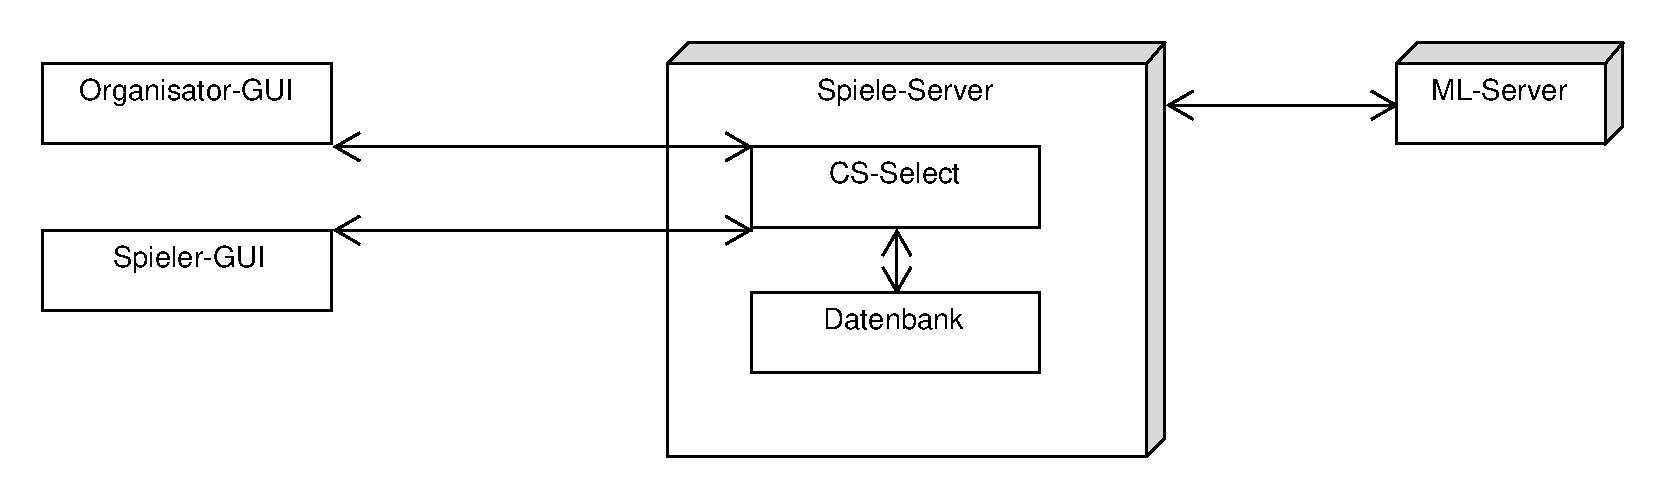
\includegraphics[scale=0.4]{img/Architektur.pdf}
\end{frame}

\begin{frame}{Ablauf der Merkmalsauswahl}
    \begin{itemize}
        \item Produkt erhält Merkmalsdatensatz vom ML-Server
        \item Spiel wird vom Organisator angelegt
        \item Spieler treffen die Merkmalsauswahl
        \item Merkmalsauswahl wird in Datenbank gesichert
    \end{itemize}
\end{frame}
\begin{frame}{Merkmalsauswahl - Spielmodi}
    \begin{columns}
        \begin{column}{0.5\textwidth}
            \begin{block}{Matrix-Select}
                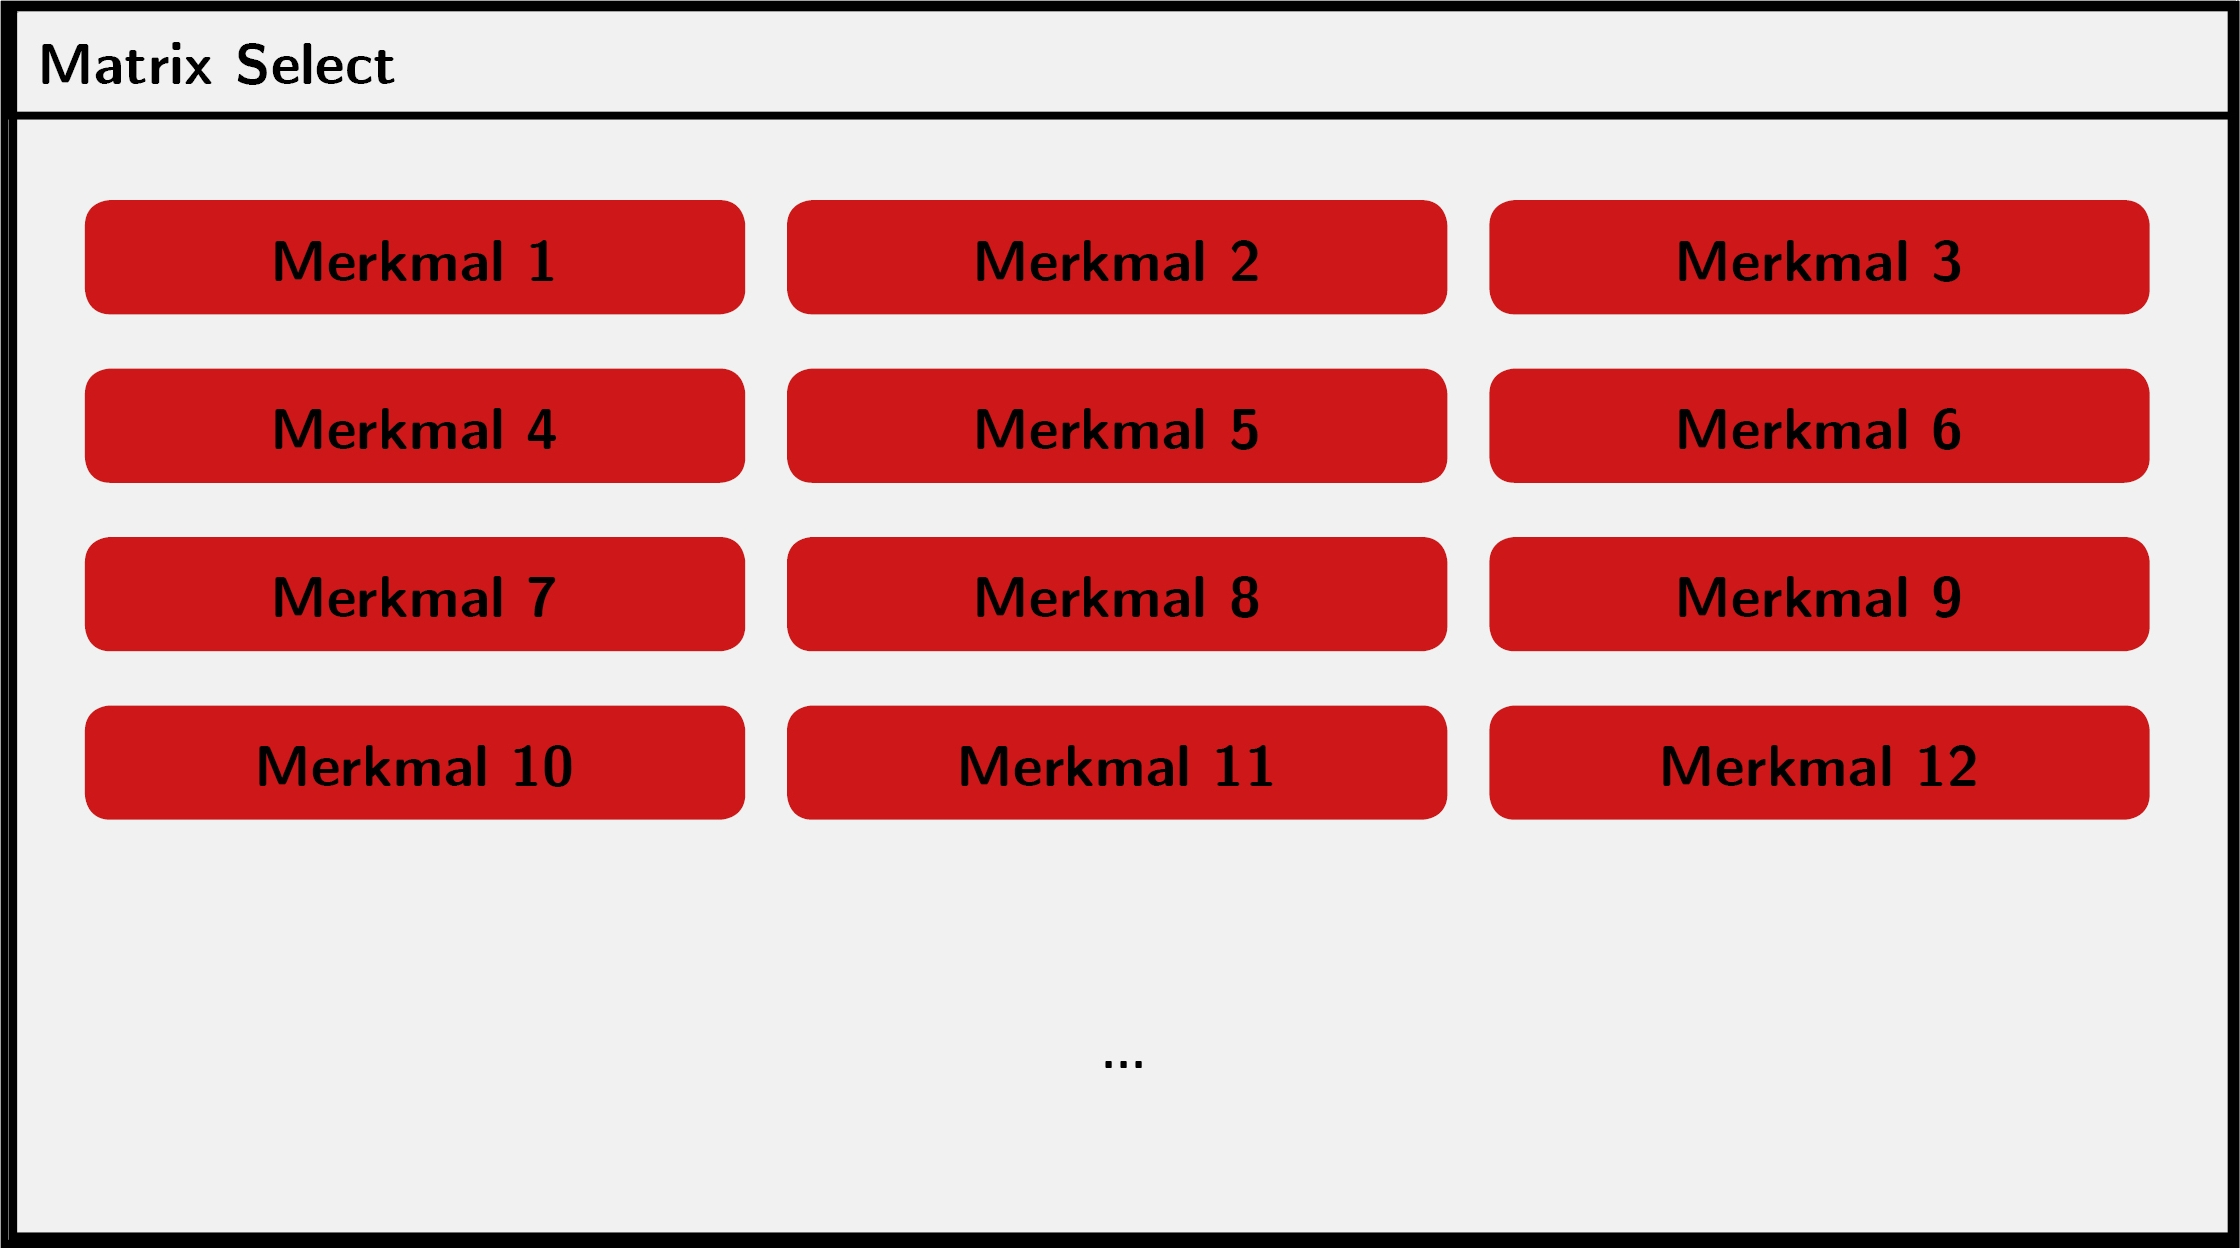
\includegraphics[width=\textwidth]{img/MatrixSelect_ausschnitt.jpg}
            \end{block}
        \end{column}
        \begin{column}{0.5\textwidth}  %%<--- here
            \begin{block}{Binär-Select}
                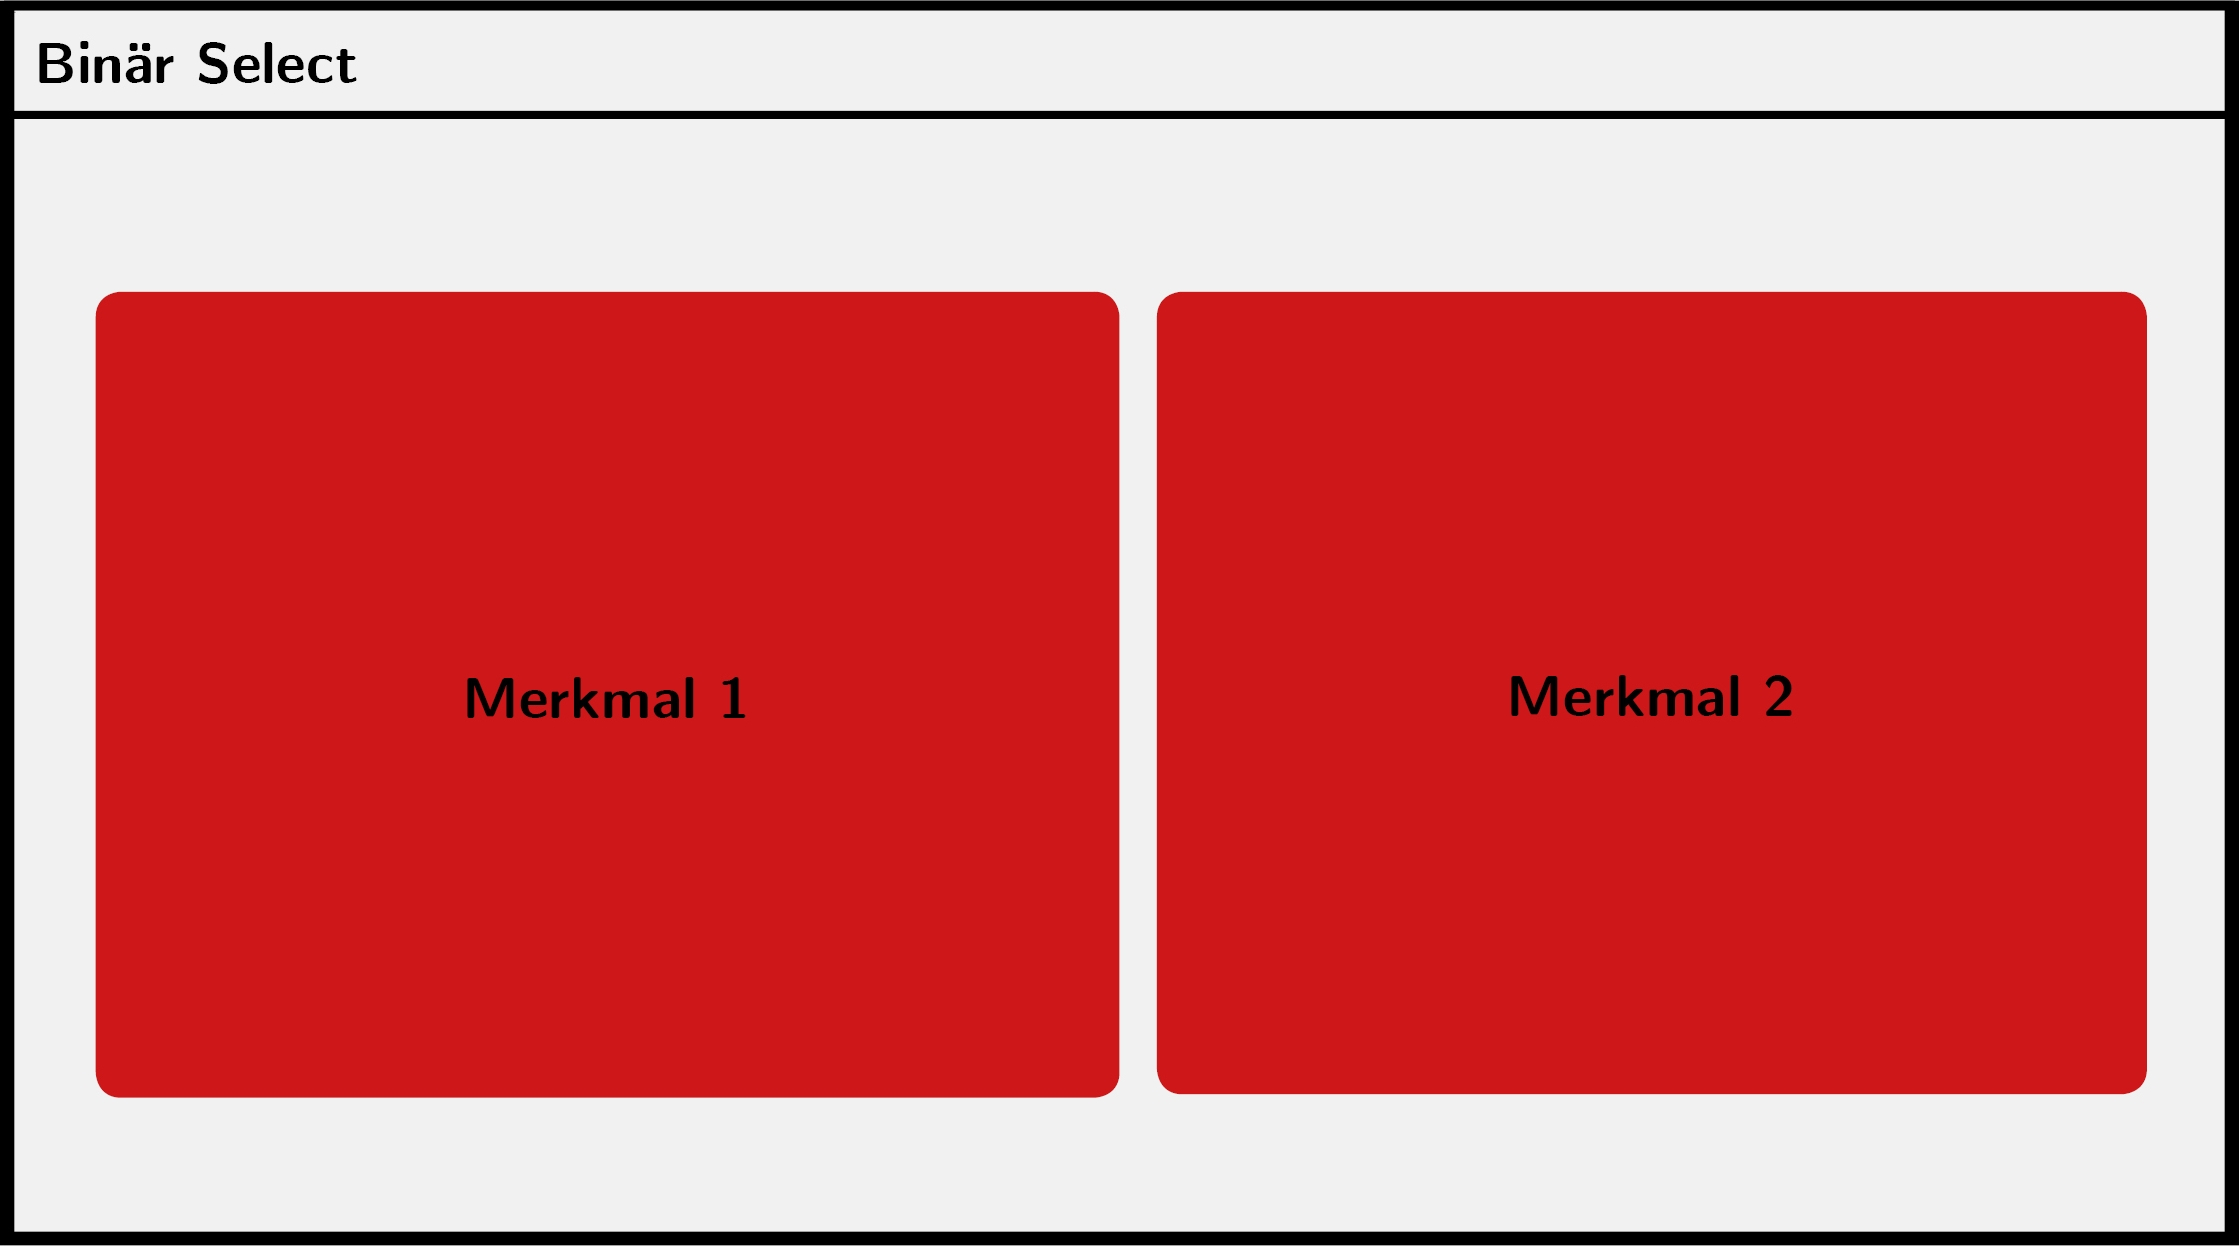
\includegraphics[width=\textwidth]{img/BinSelect_ausschnitt.jpg}
            \end{block}
        \end{column}
    \end{columns}
\end{frame}
\begin{frame}{Geplante Gamification-Elemente}
    \begin{itemize}
        \item Punktesystem
        \item Leaderboard
        \item Achievements
        \item Daily Challenges
        \item Streaks
    \end{itemize}
\end{frame}
\section{Technische Grundlagen}
\againframe<1>{architektur}
\begin{frame}{Spiele-Server}
\begin{columns}
\begin{column}{0.5\textwidth}
         \begin{block}{CS-Select}
                \center
                
\includegraphics[height=4cm]{img/java.png}\\
                
\includegraphics[width=(\textwidth) / 2]{img/tomcat.png}
                Tomcat
            \end{block} 
\end{column}
\begin{column}{0.5\textwidth}  %%<--- here
        \begin{block}{Datenbank}
                
\includegraphics[width=\textwidth]{img/MySQL.jpg}
    \end{block}
\end{column}
\end{columns}
\end{frame}
\againframe<2>{architektur}
\begin{frame}{Grafische Nutzerschnittstelle}
        
\includegraphics[width=5cm]{img/vue.png}
        \begin{block}{Interface}
        Vue.js Framework
        \end{block}
\end{frame}
\againframe<3>{architektur}
\begin{frame}{Optional}
         
\includegraphics[width=5cm]{img/docker.jpg}
         \begin{block}{Optional}
          Produkt als Docker Container liefern.
        \end{block}
\end{frame}
\section{Testfallszenarien}
    \subsection{Organisator-Testkette}
    \begin{frame}
        \begin{block} {Anmeldung, Spielerstellung}
            Der Organisator möchte sich auf dem Spiel-Server anmelden und ein neues Spiel erstellen.
        \end{block}
        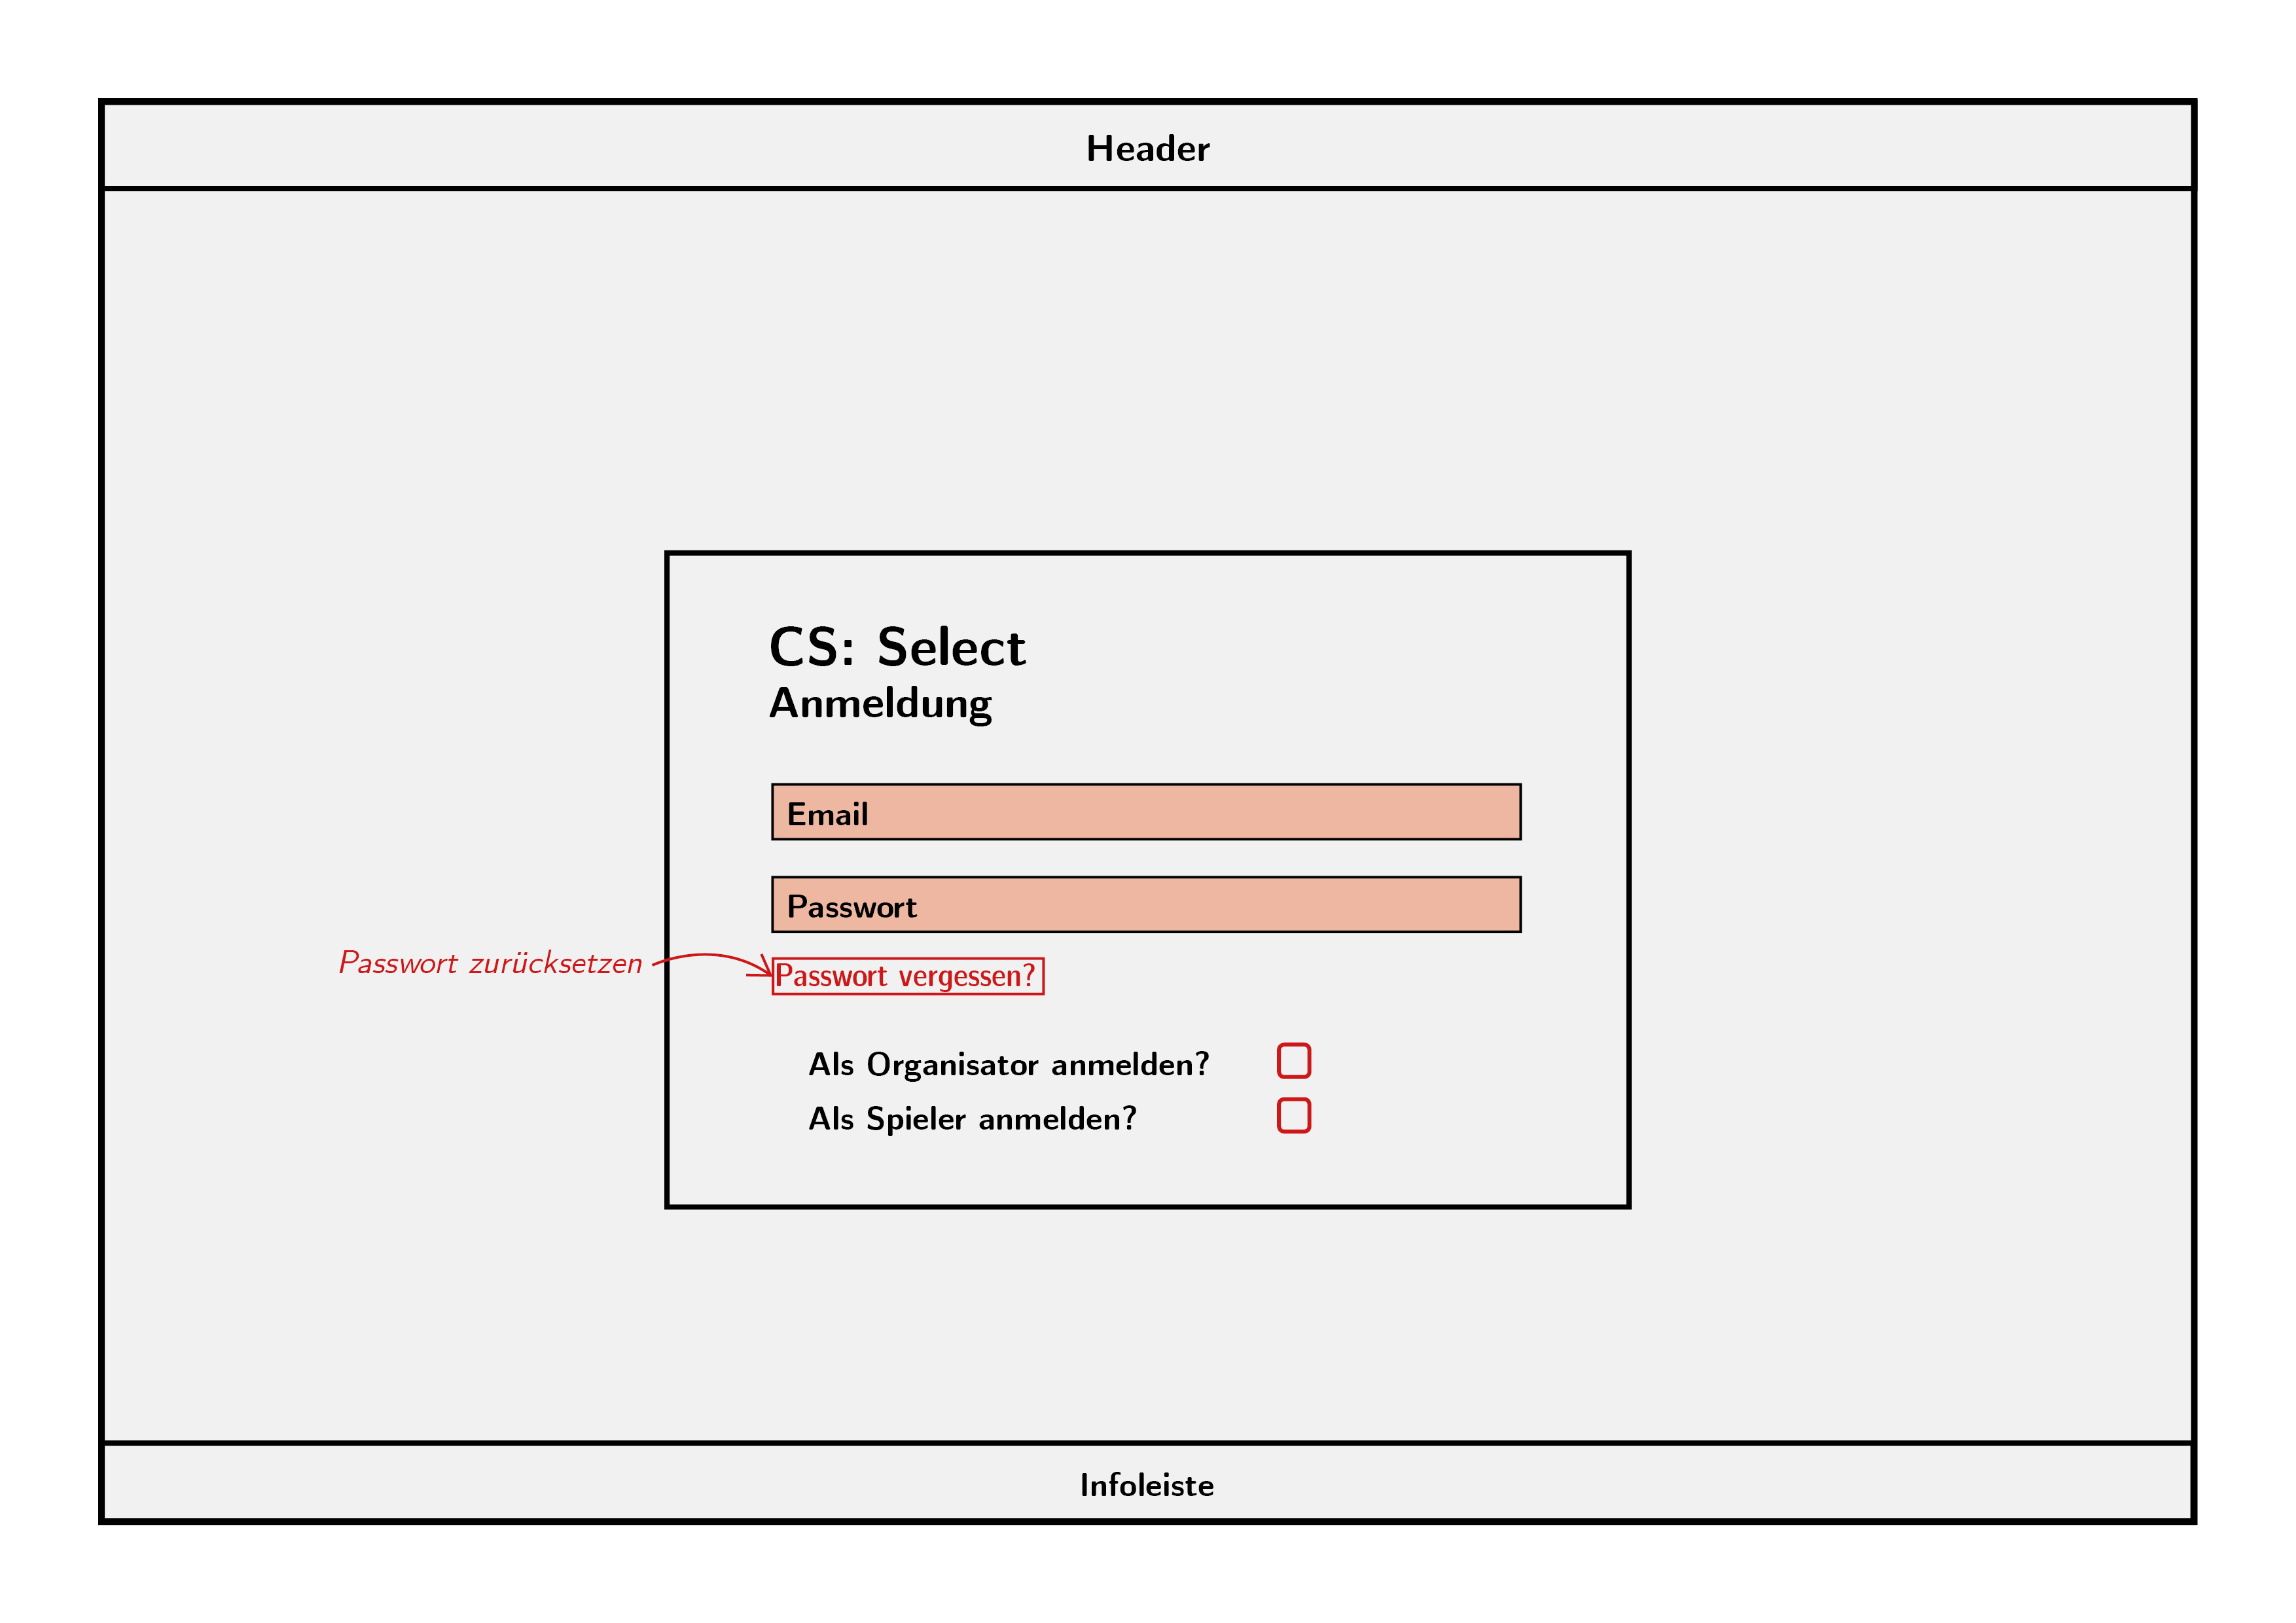
\includegraphics[width=8cm]{img/Anmeldung.jpg}
    \end{frame}
    \begin{frame}
        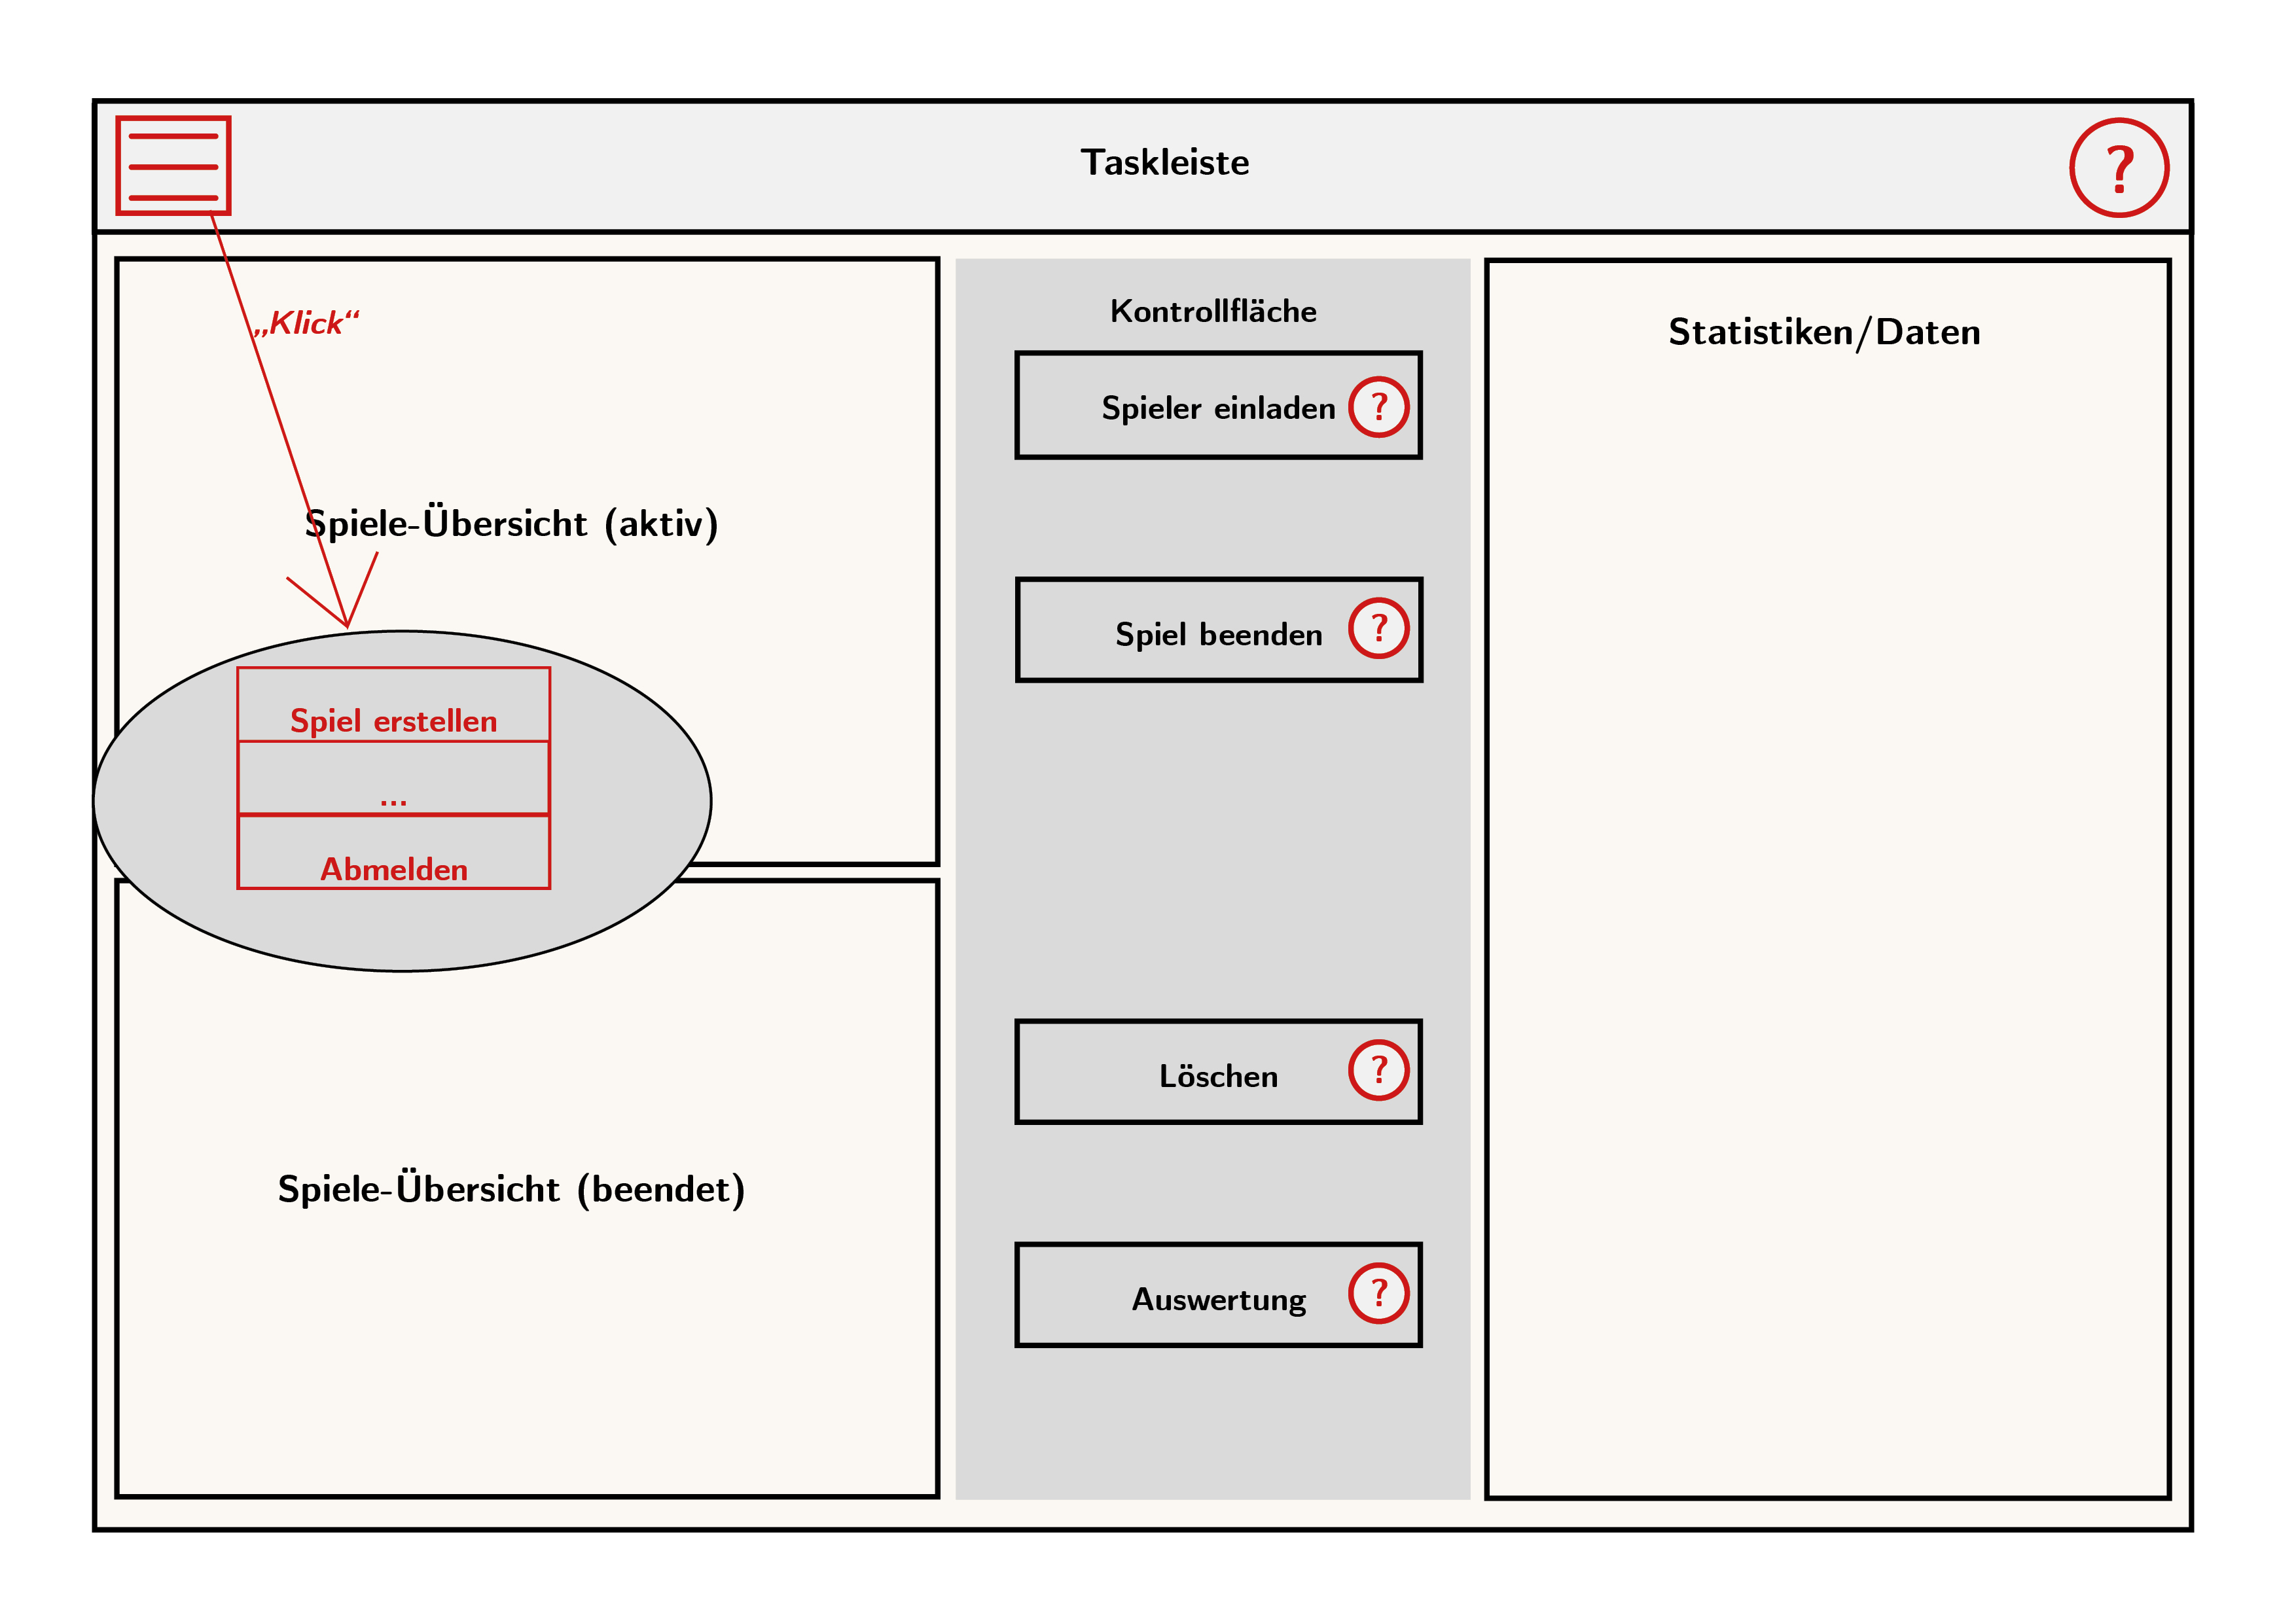
\includegraphics[width=\textwidth]{img/OrganisatorPres.jpg}
    \end{frame}
    \begin{frame}
         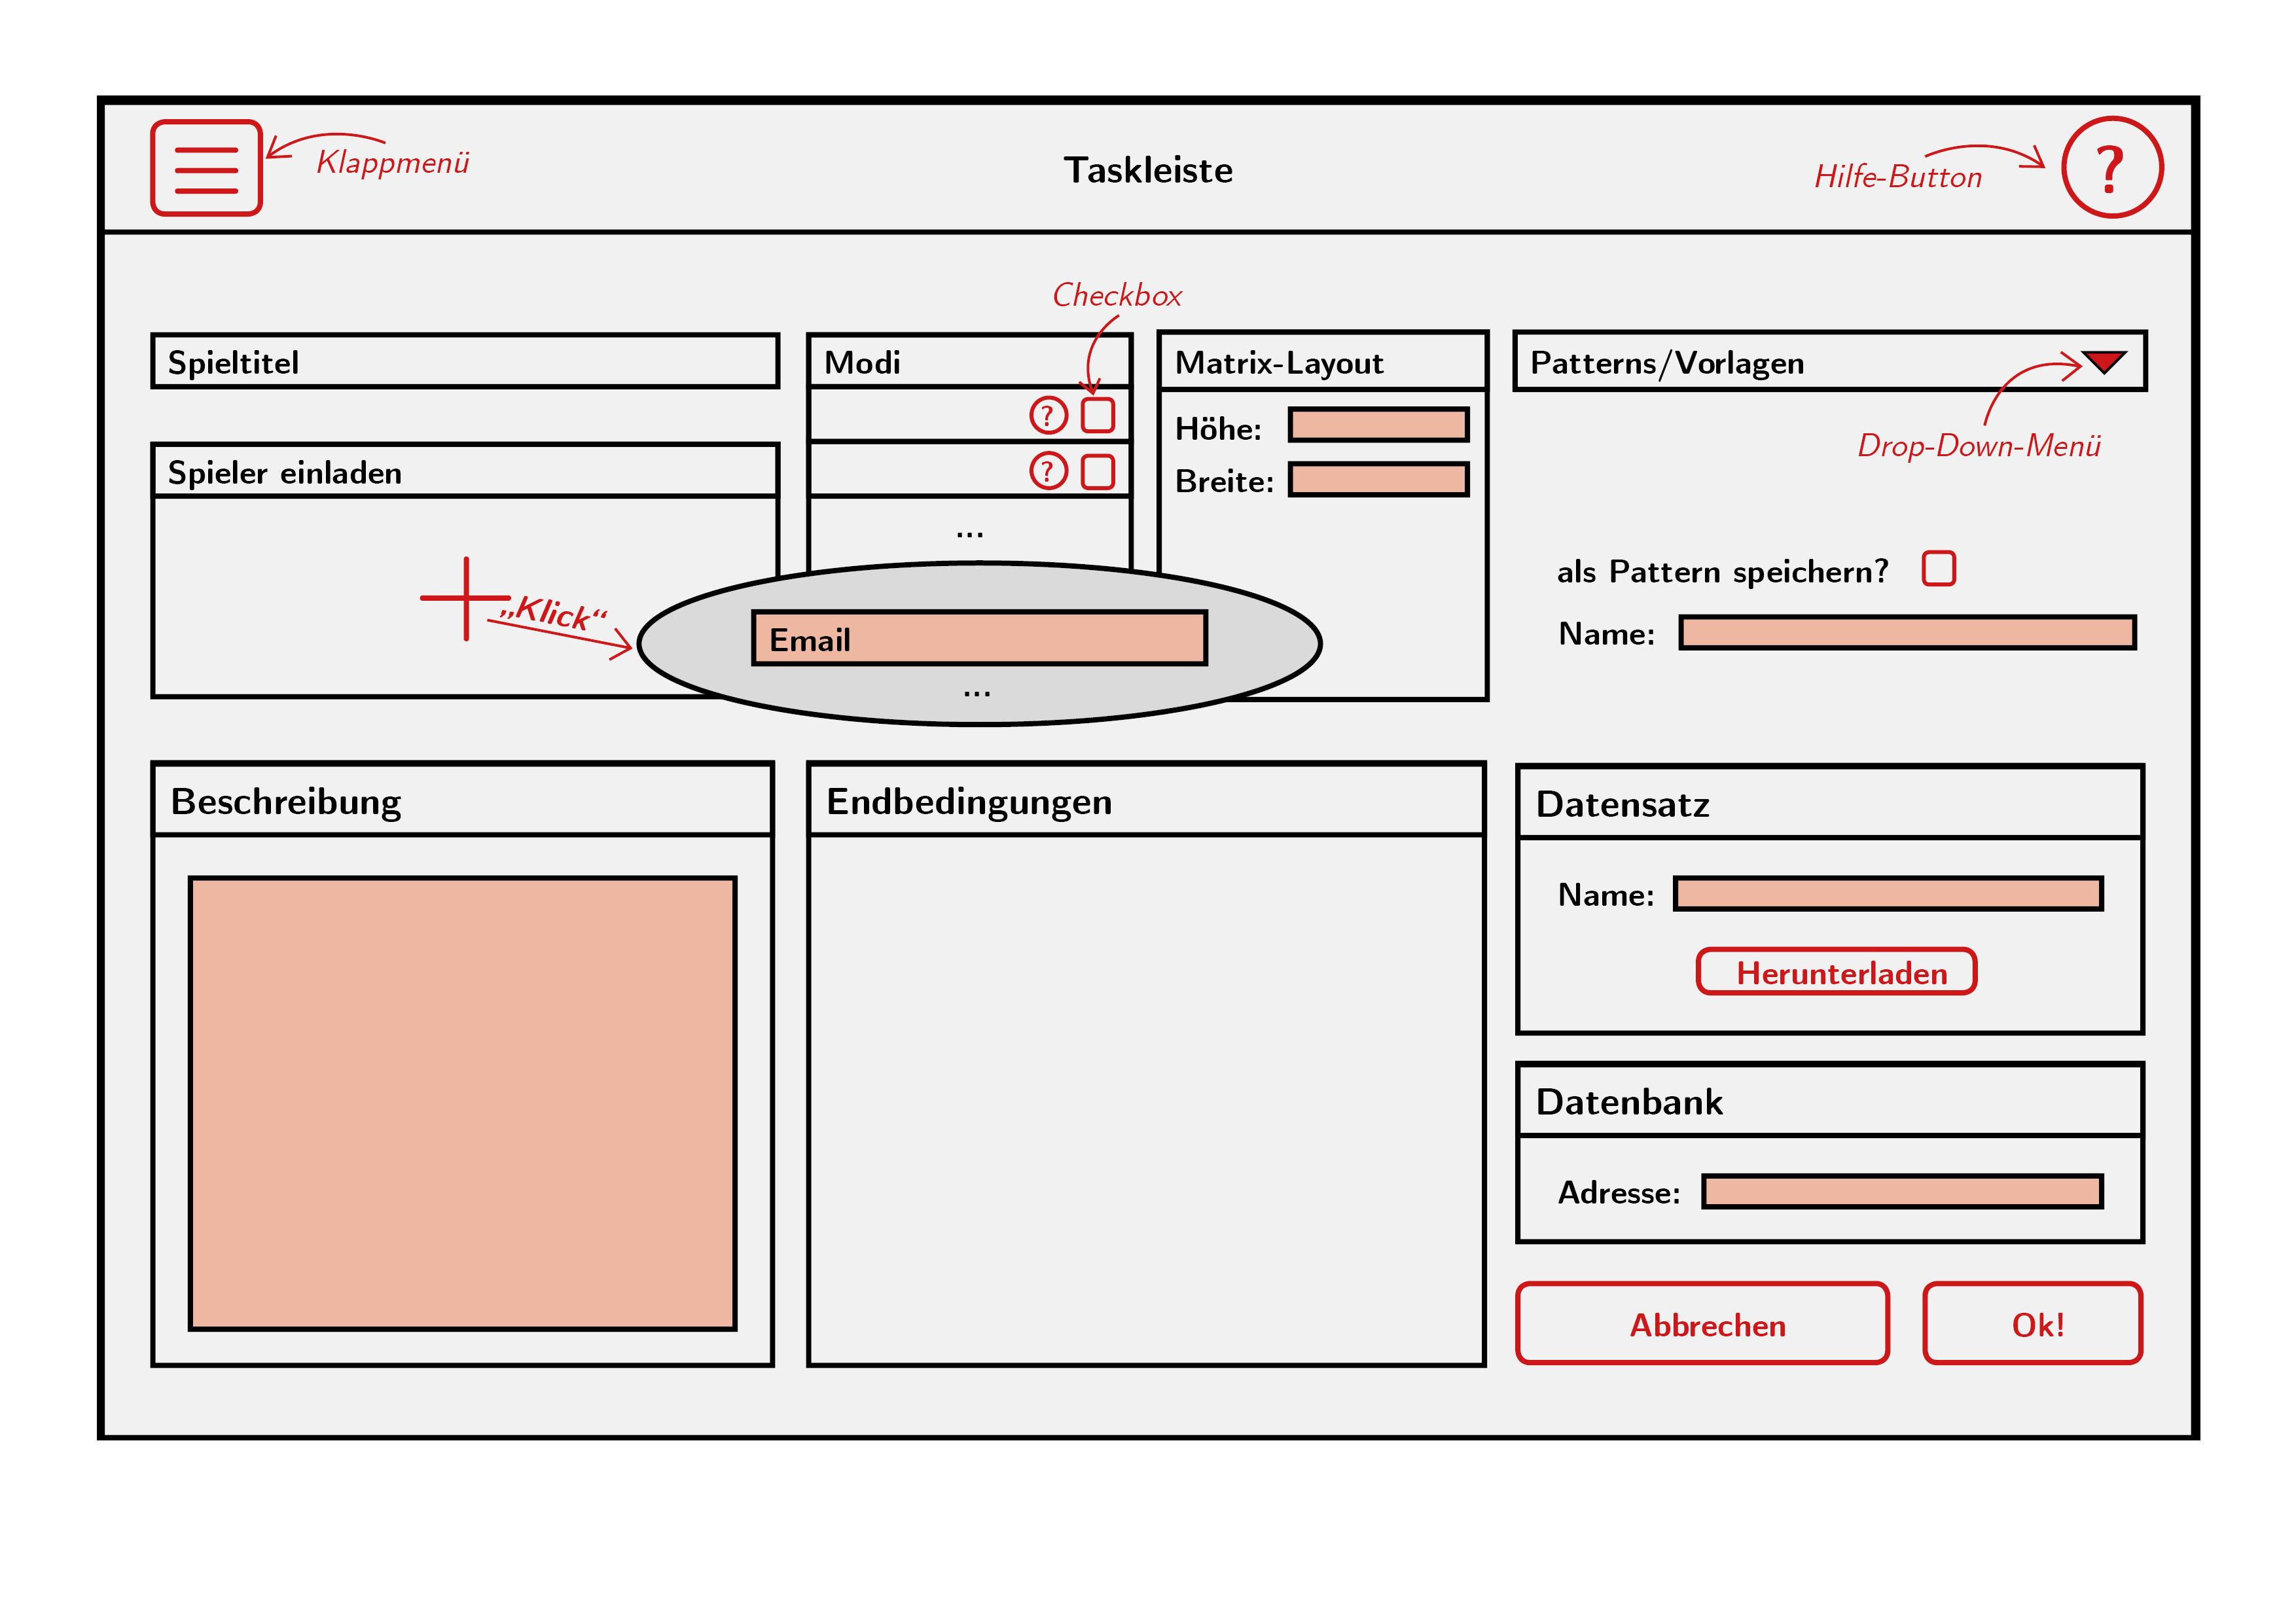
\includegraphics[width=\textwidth]{img/Spielerstellung.jpg}
    \end{frame}
    \begin{frame}
        \begin{block} {Spieler nachträglich einladen, Spiel beenden}
            Nun wird der Organisator einen neuen Spieler zum eben erstellten Spiel einladen und ein anderes aktives Spiel beenden.
        \end{block}
        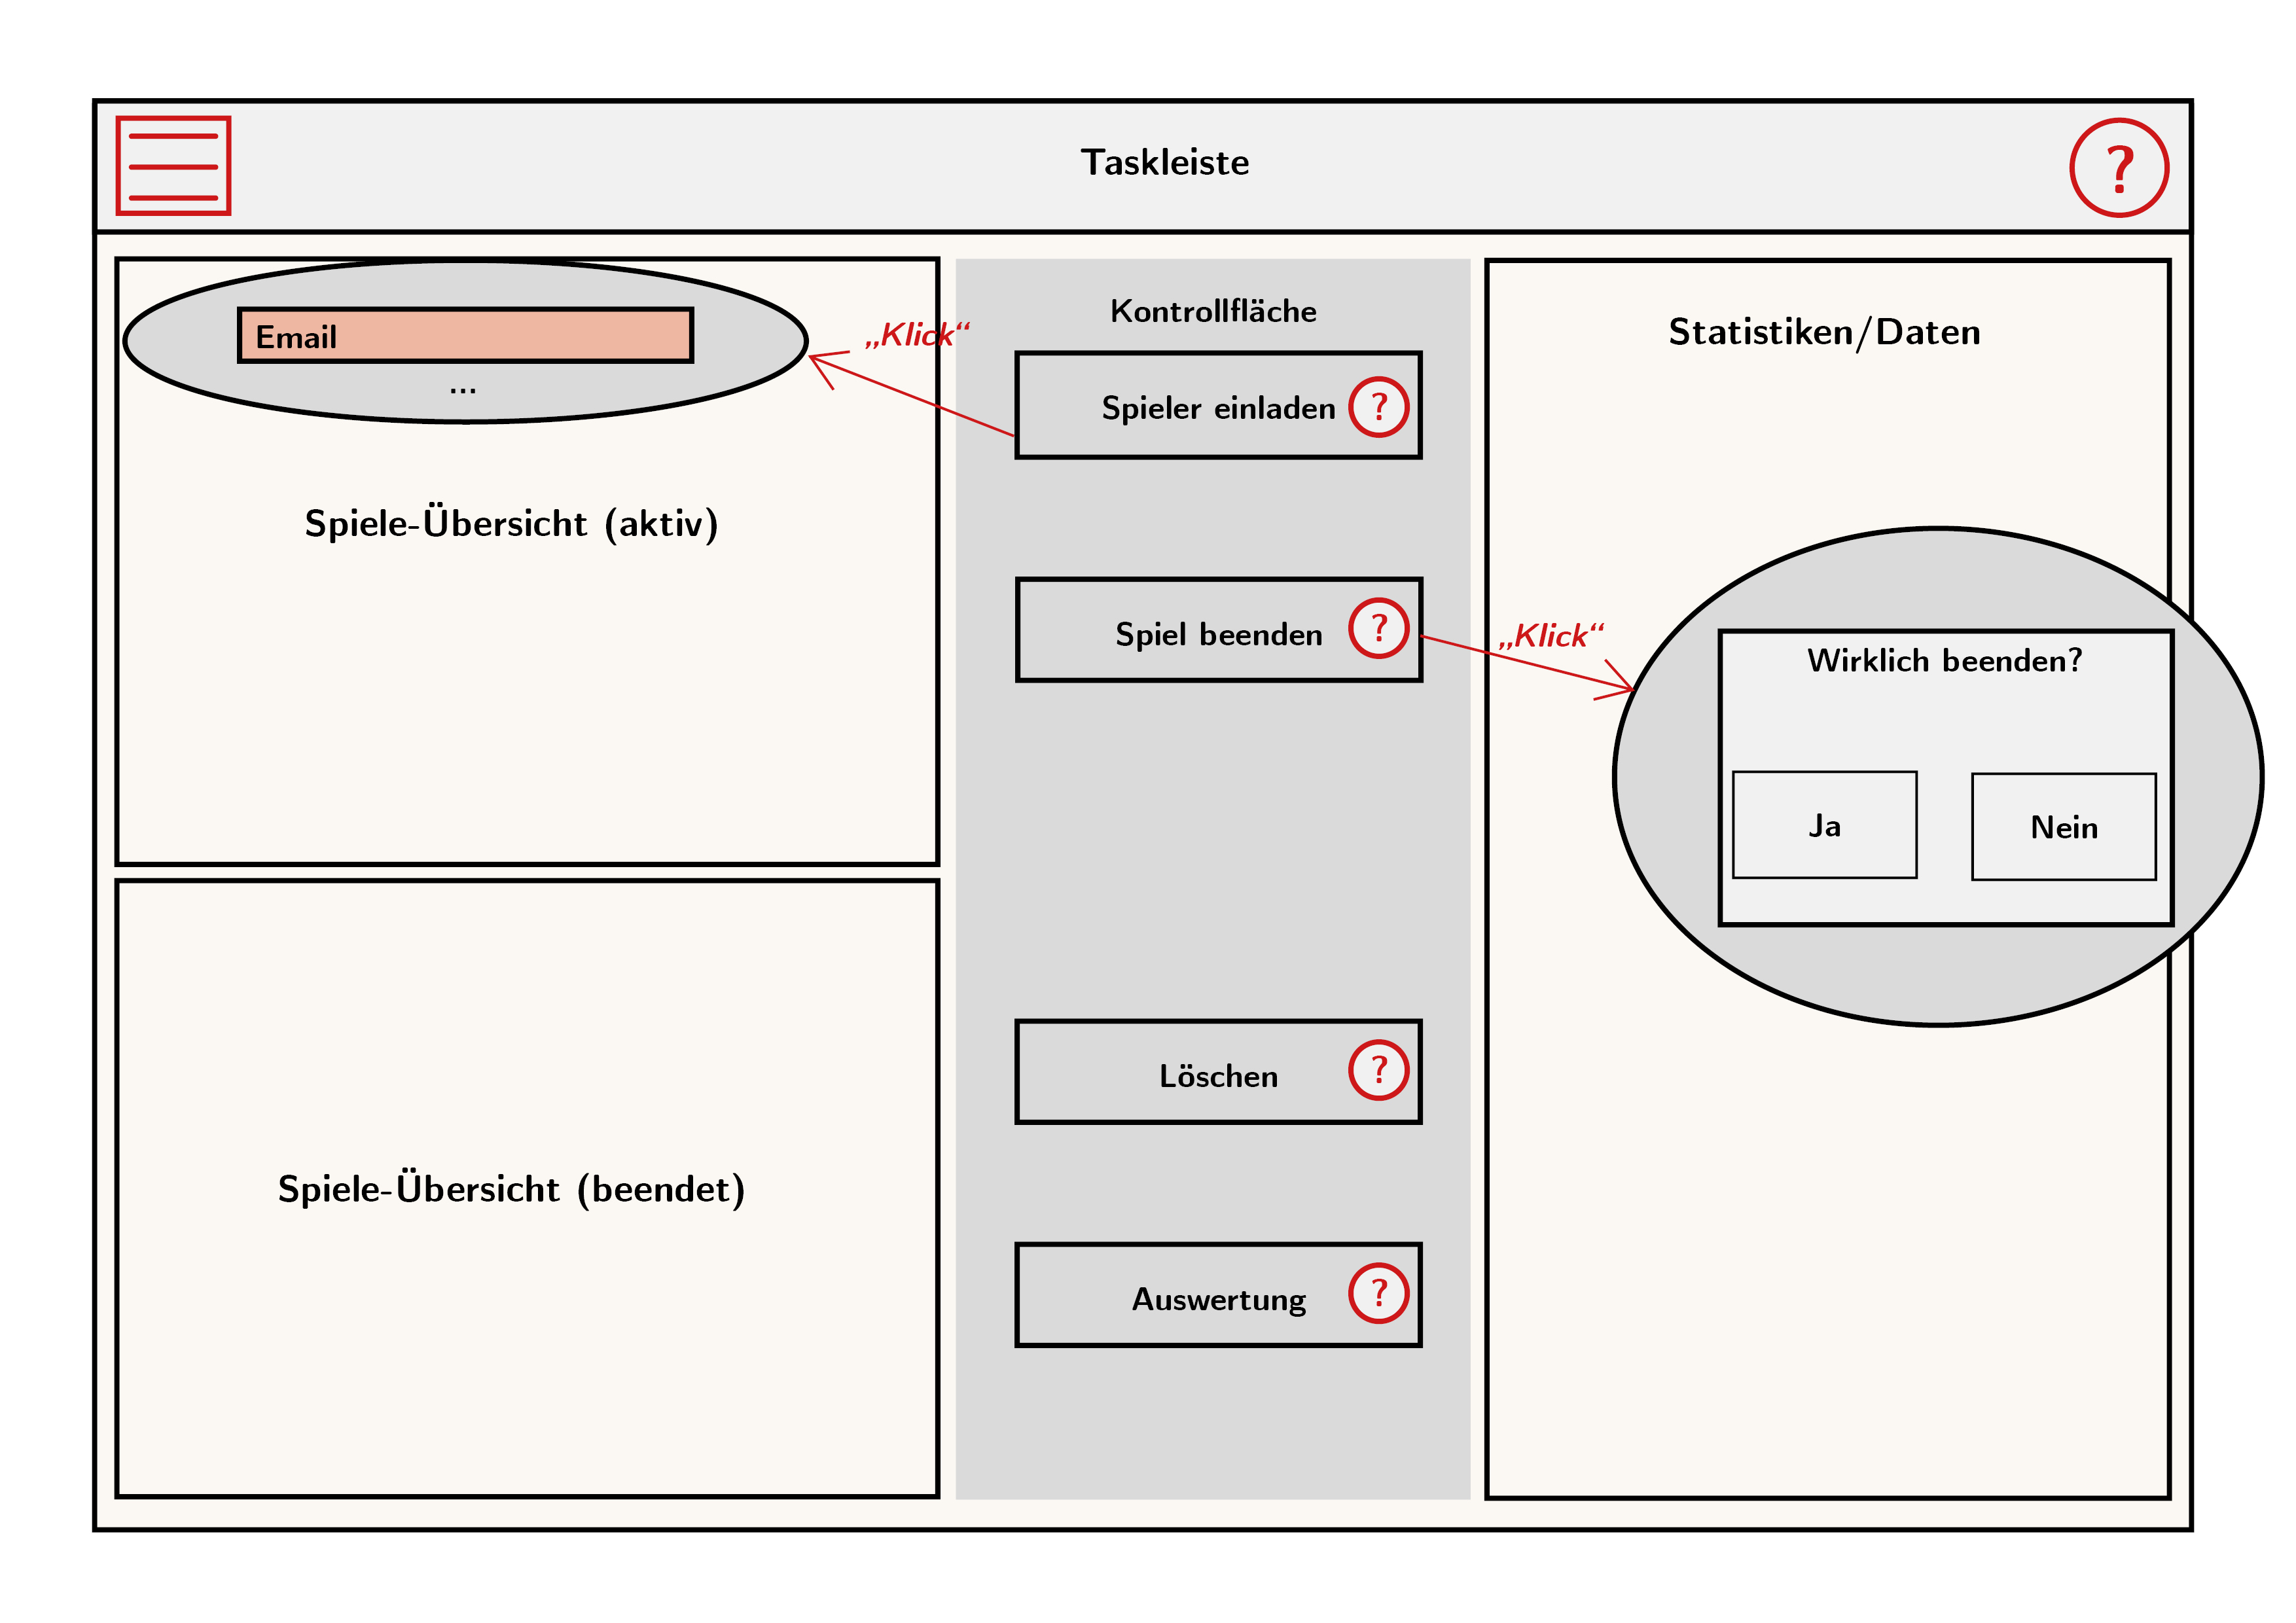
\includegraphics[width=8cm]{img/OrganisatorPres2.jpg}
    \end{frame}
	\subsection{}
    \begin{frame}{Spieler-Testkette} 
    	\begin{block}{Anmeldung, Matrix Select spielen}
    		Der Spieler möchte sich auf dem Spiel-Server anmelden und eine Runde eines Spiels mit Spielmodus Matrix Select spielen.
    	\end{block}
    	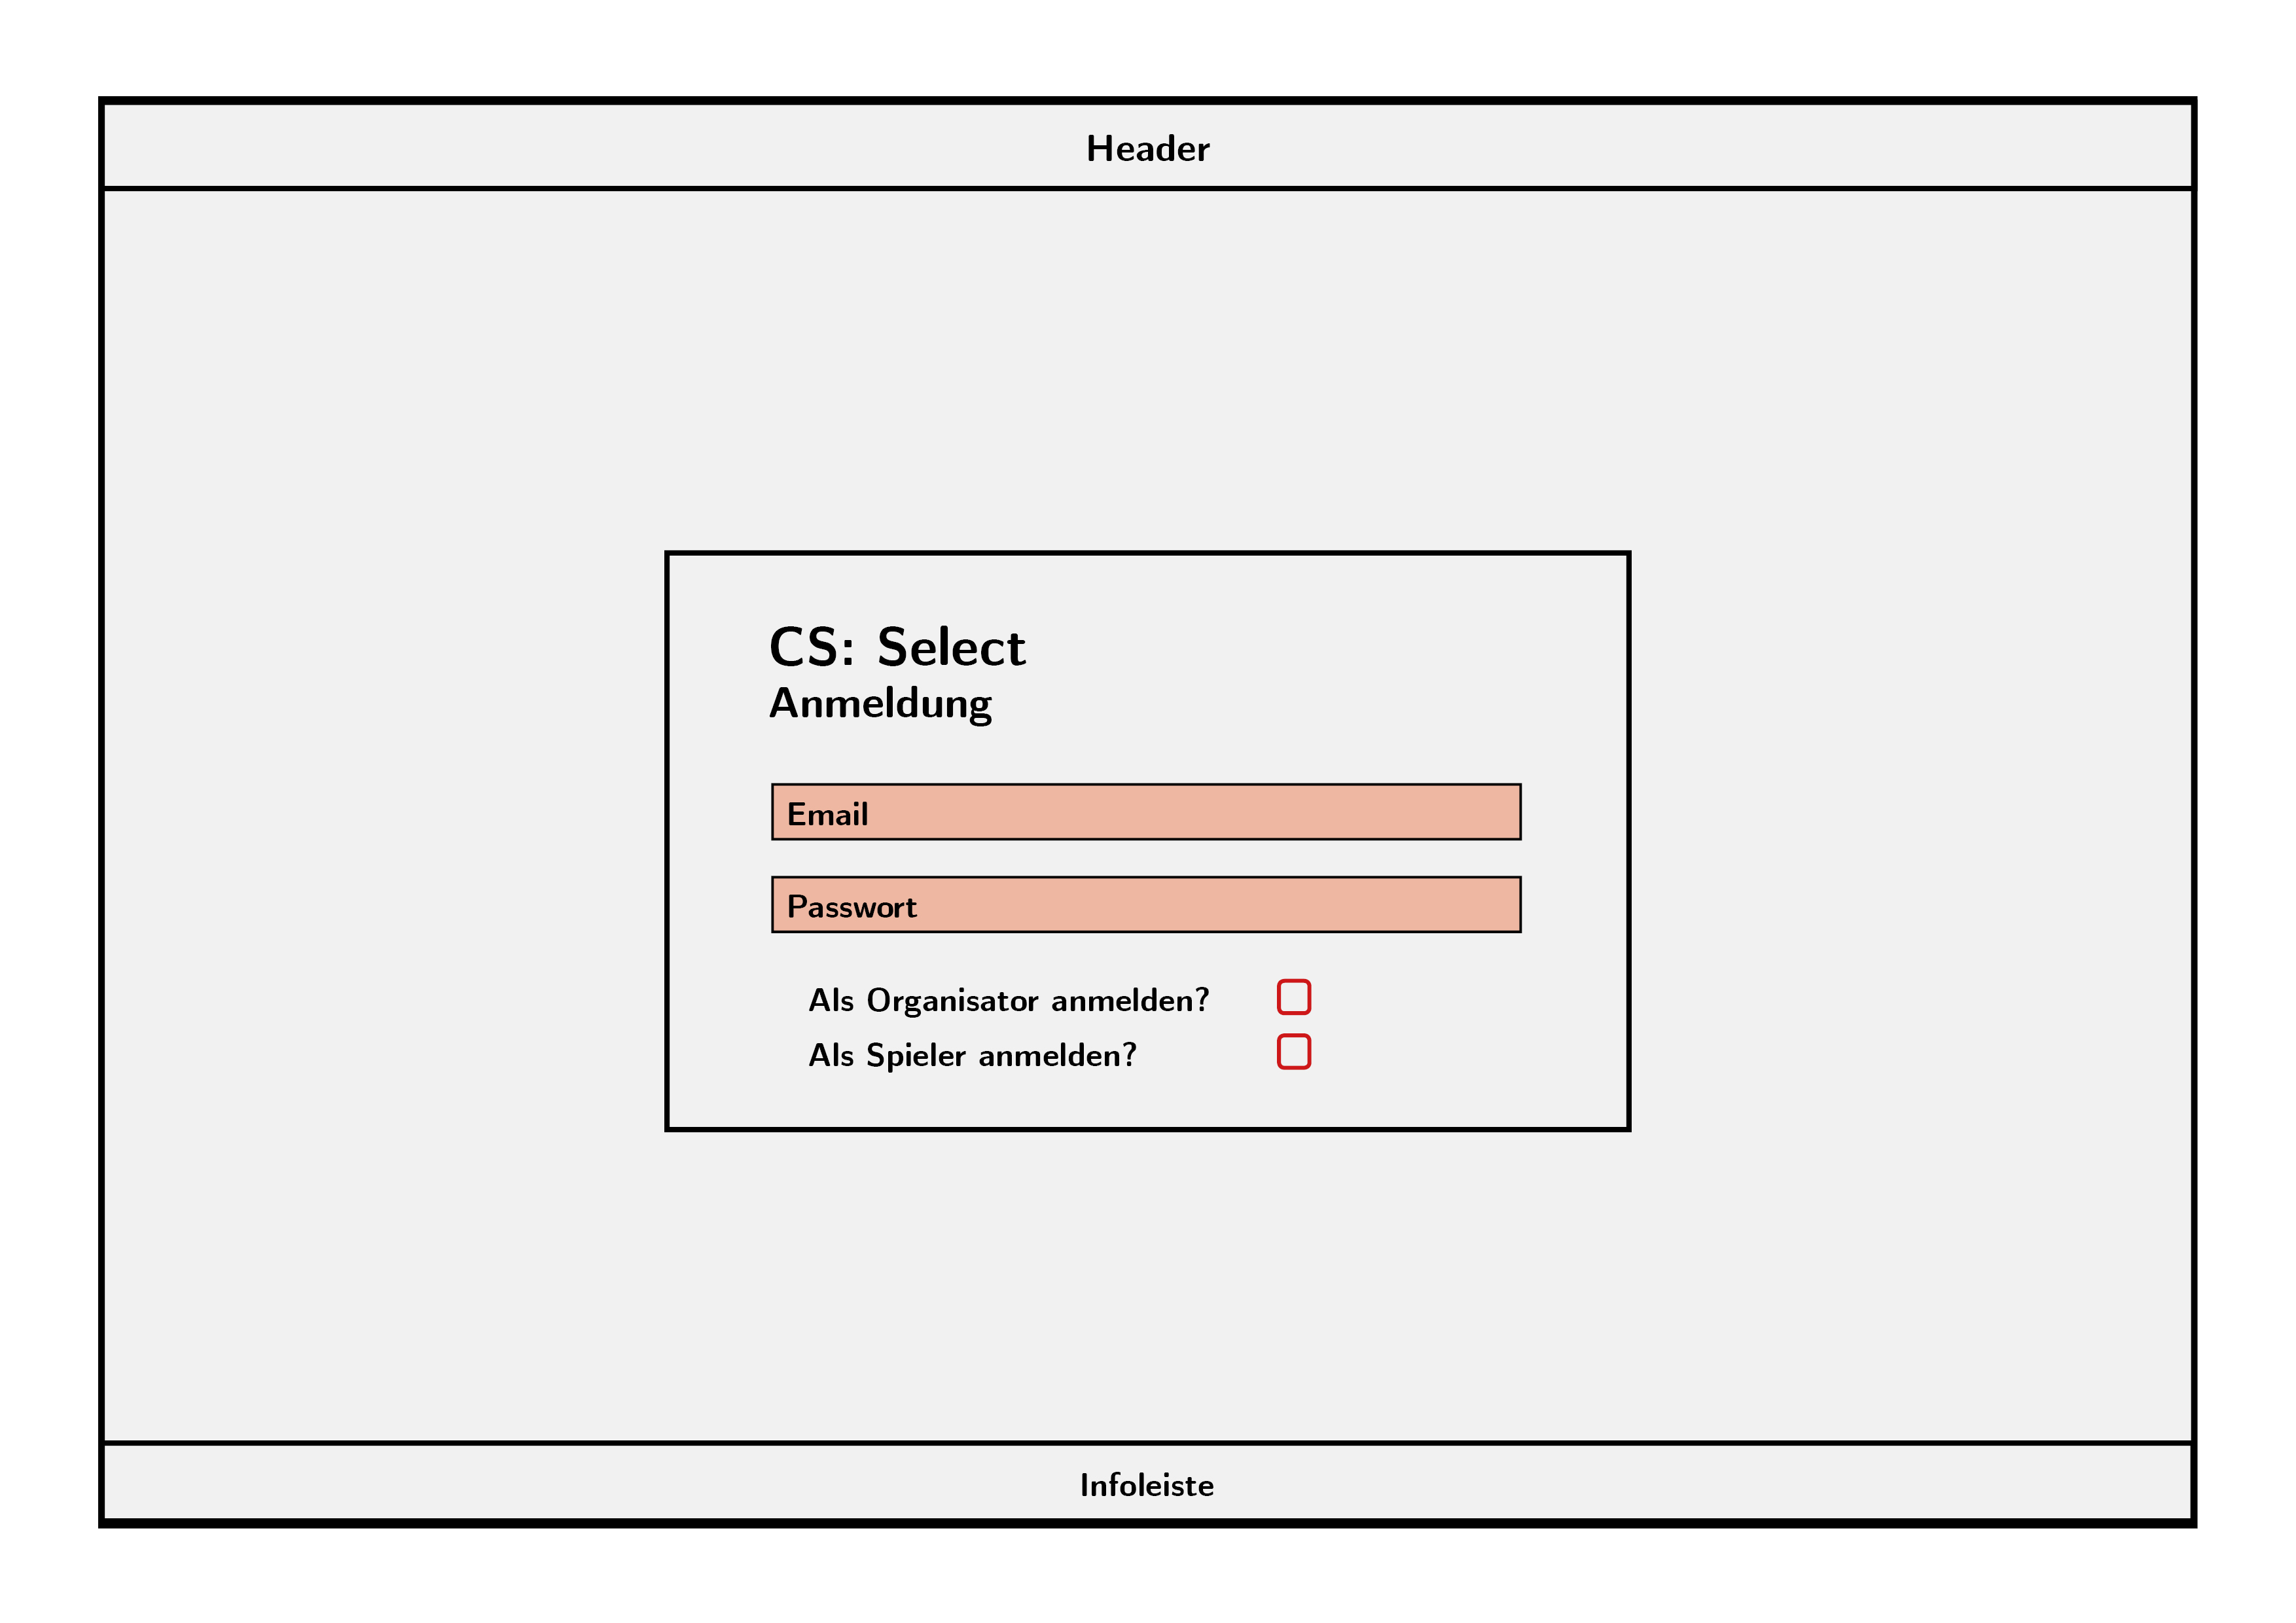
\includegraphics[width=8cm]{../../pictures/Anmeldung.jpg}
    \end{frame}
	\subsection{Spieler-Testkette} 
	\begin{frame}
	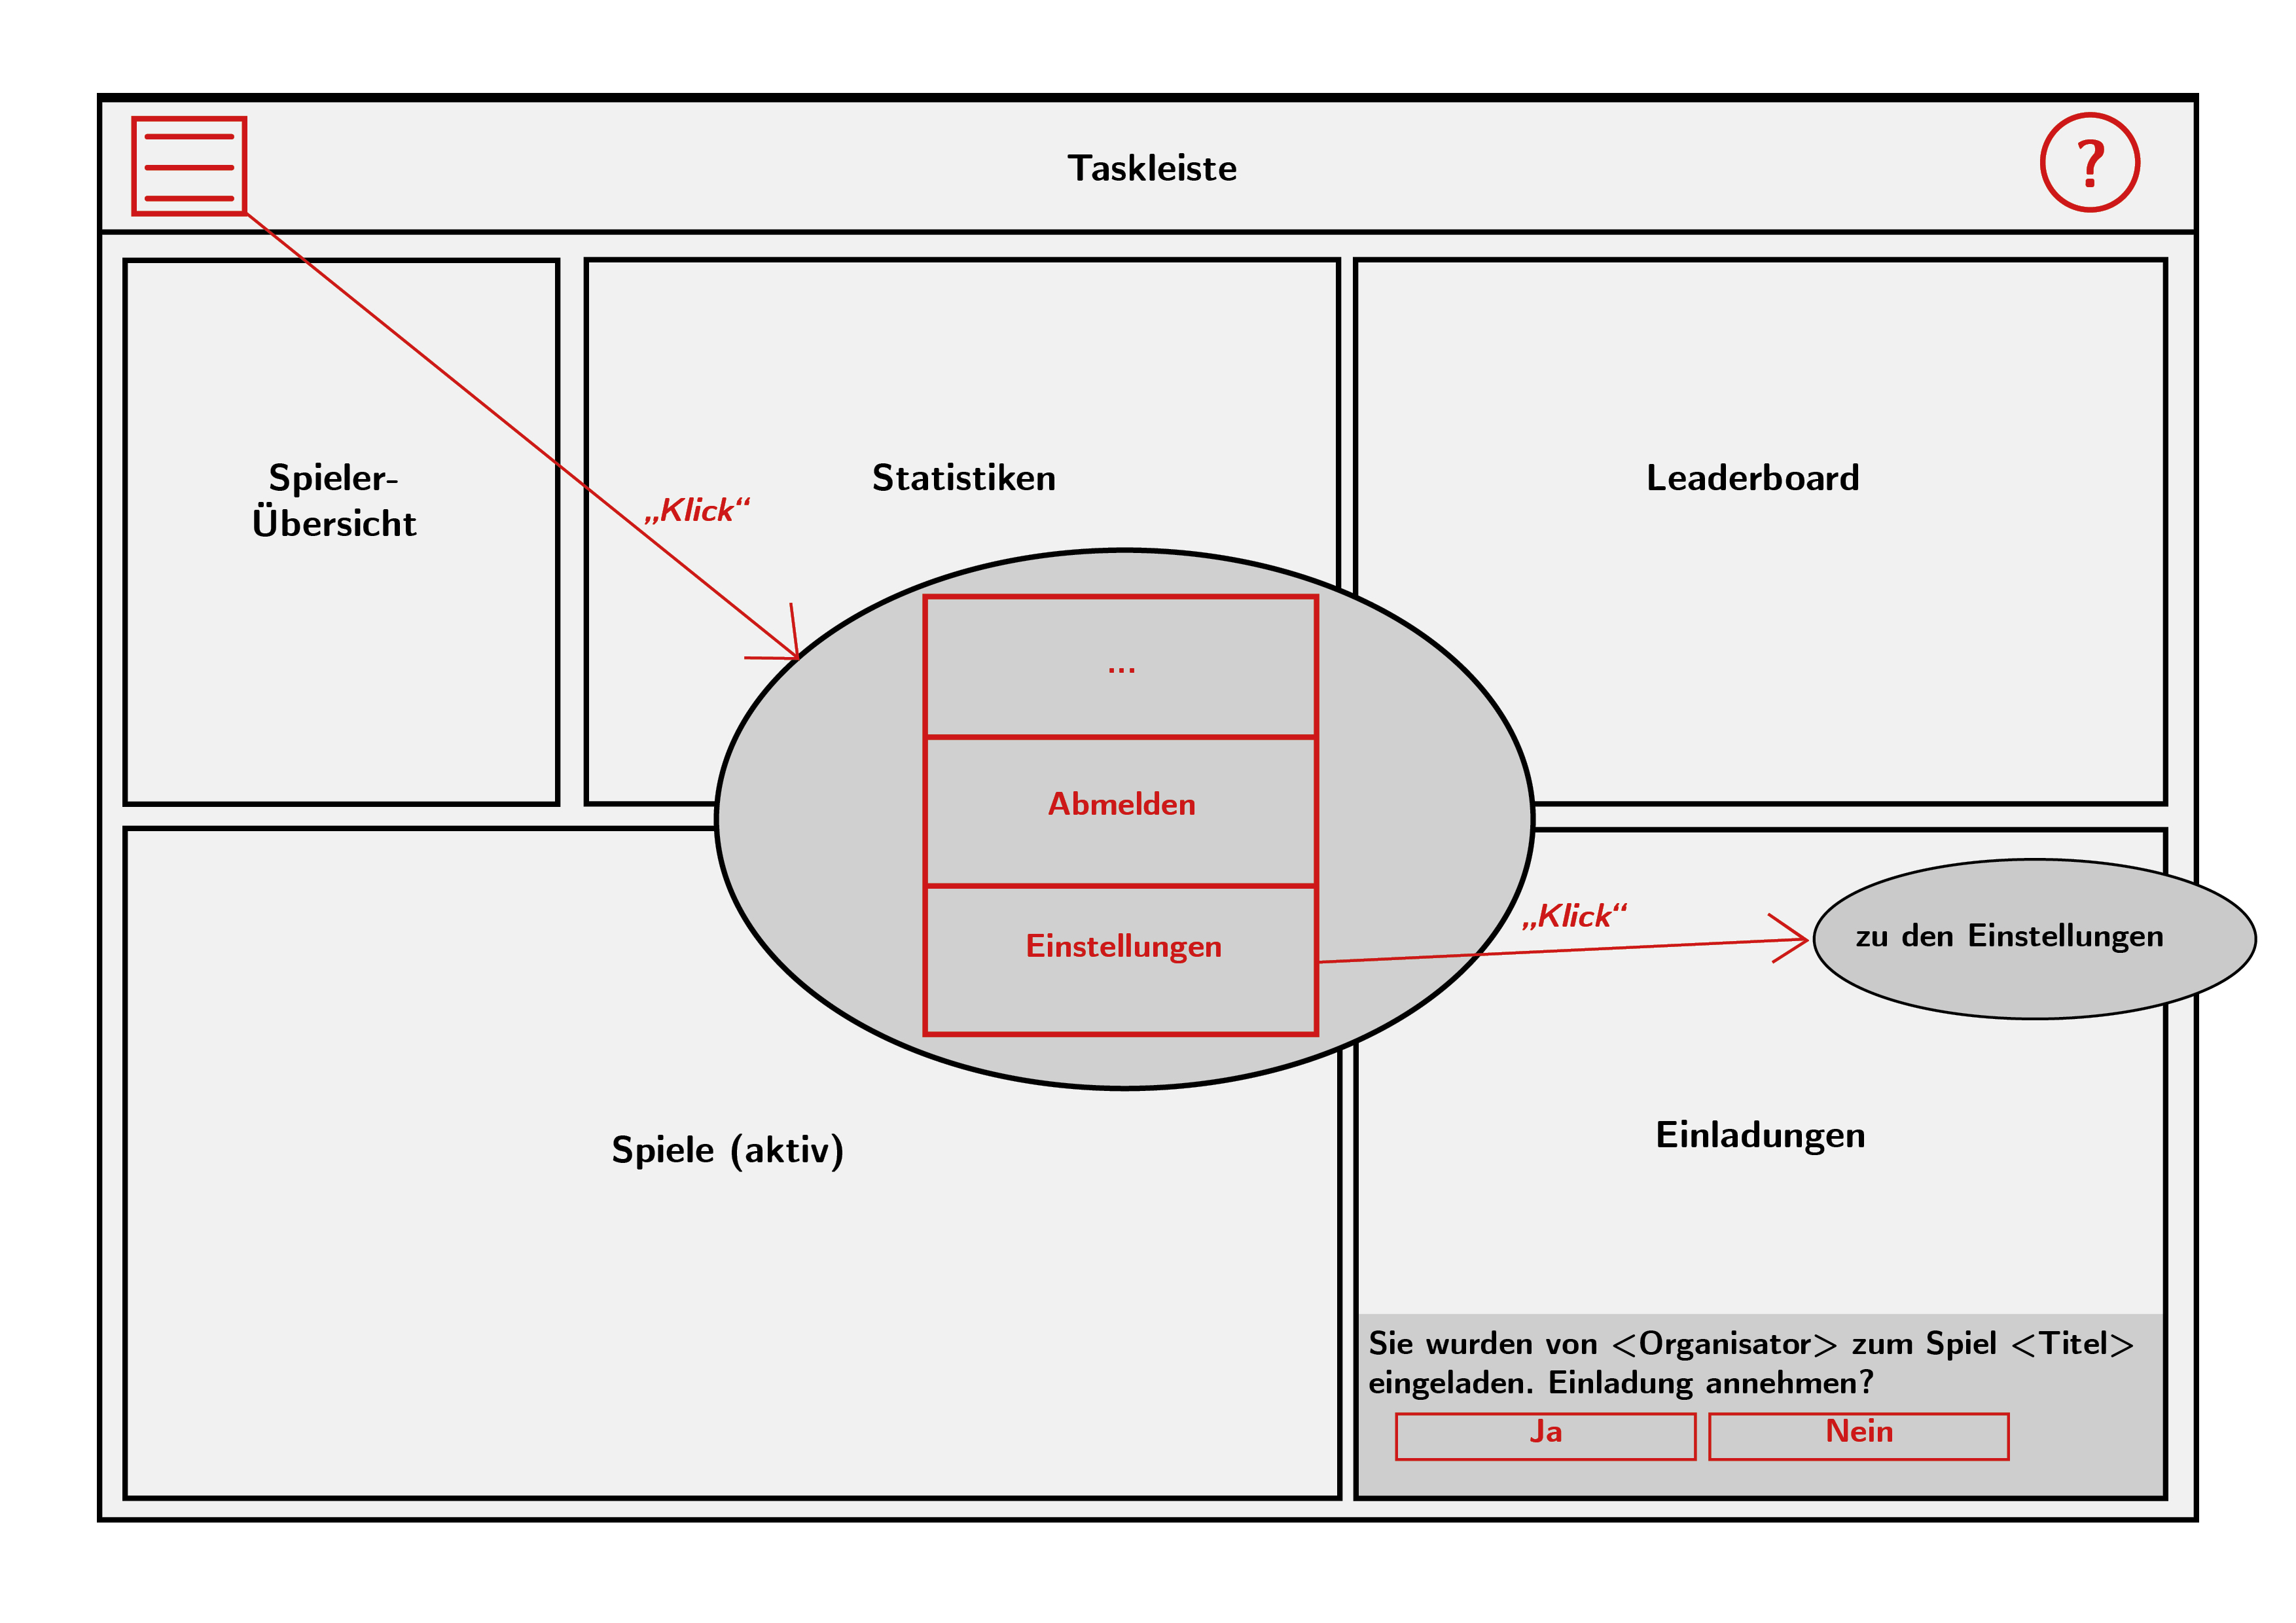
\includegraphics[width=\textwidth]{../../pictures/5_Spieler.jpg}
	\end{frame}
	\begin{frame}
	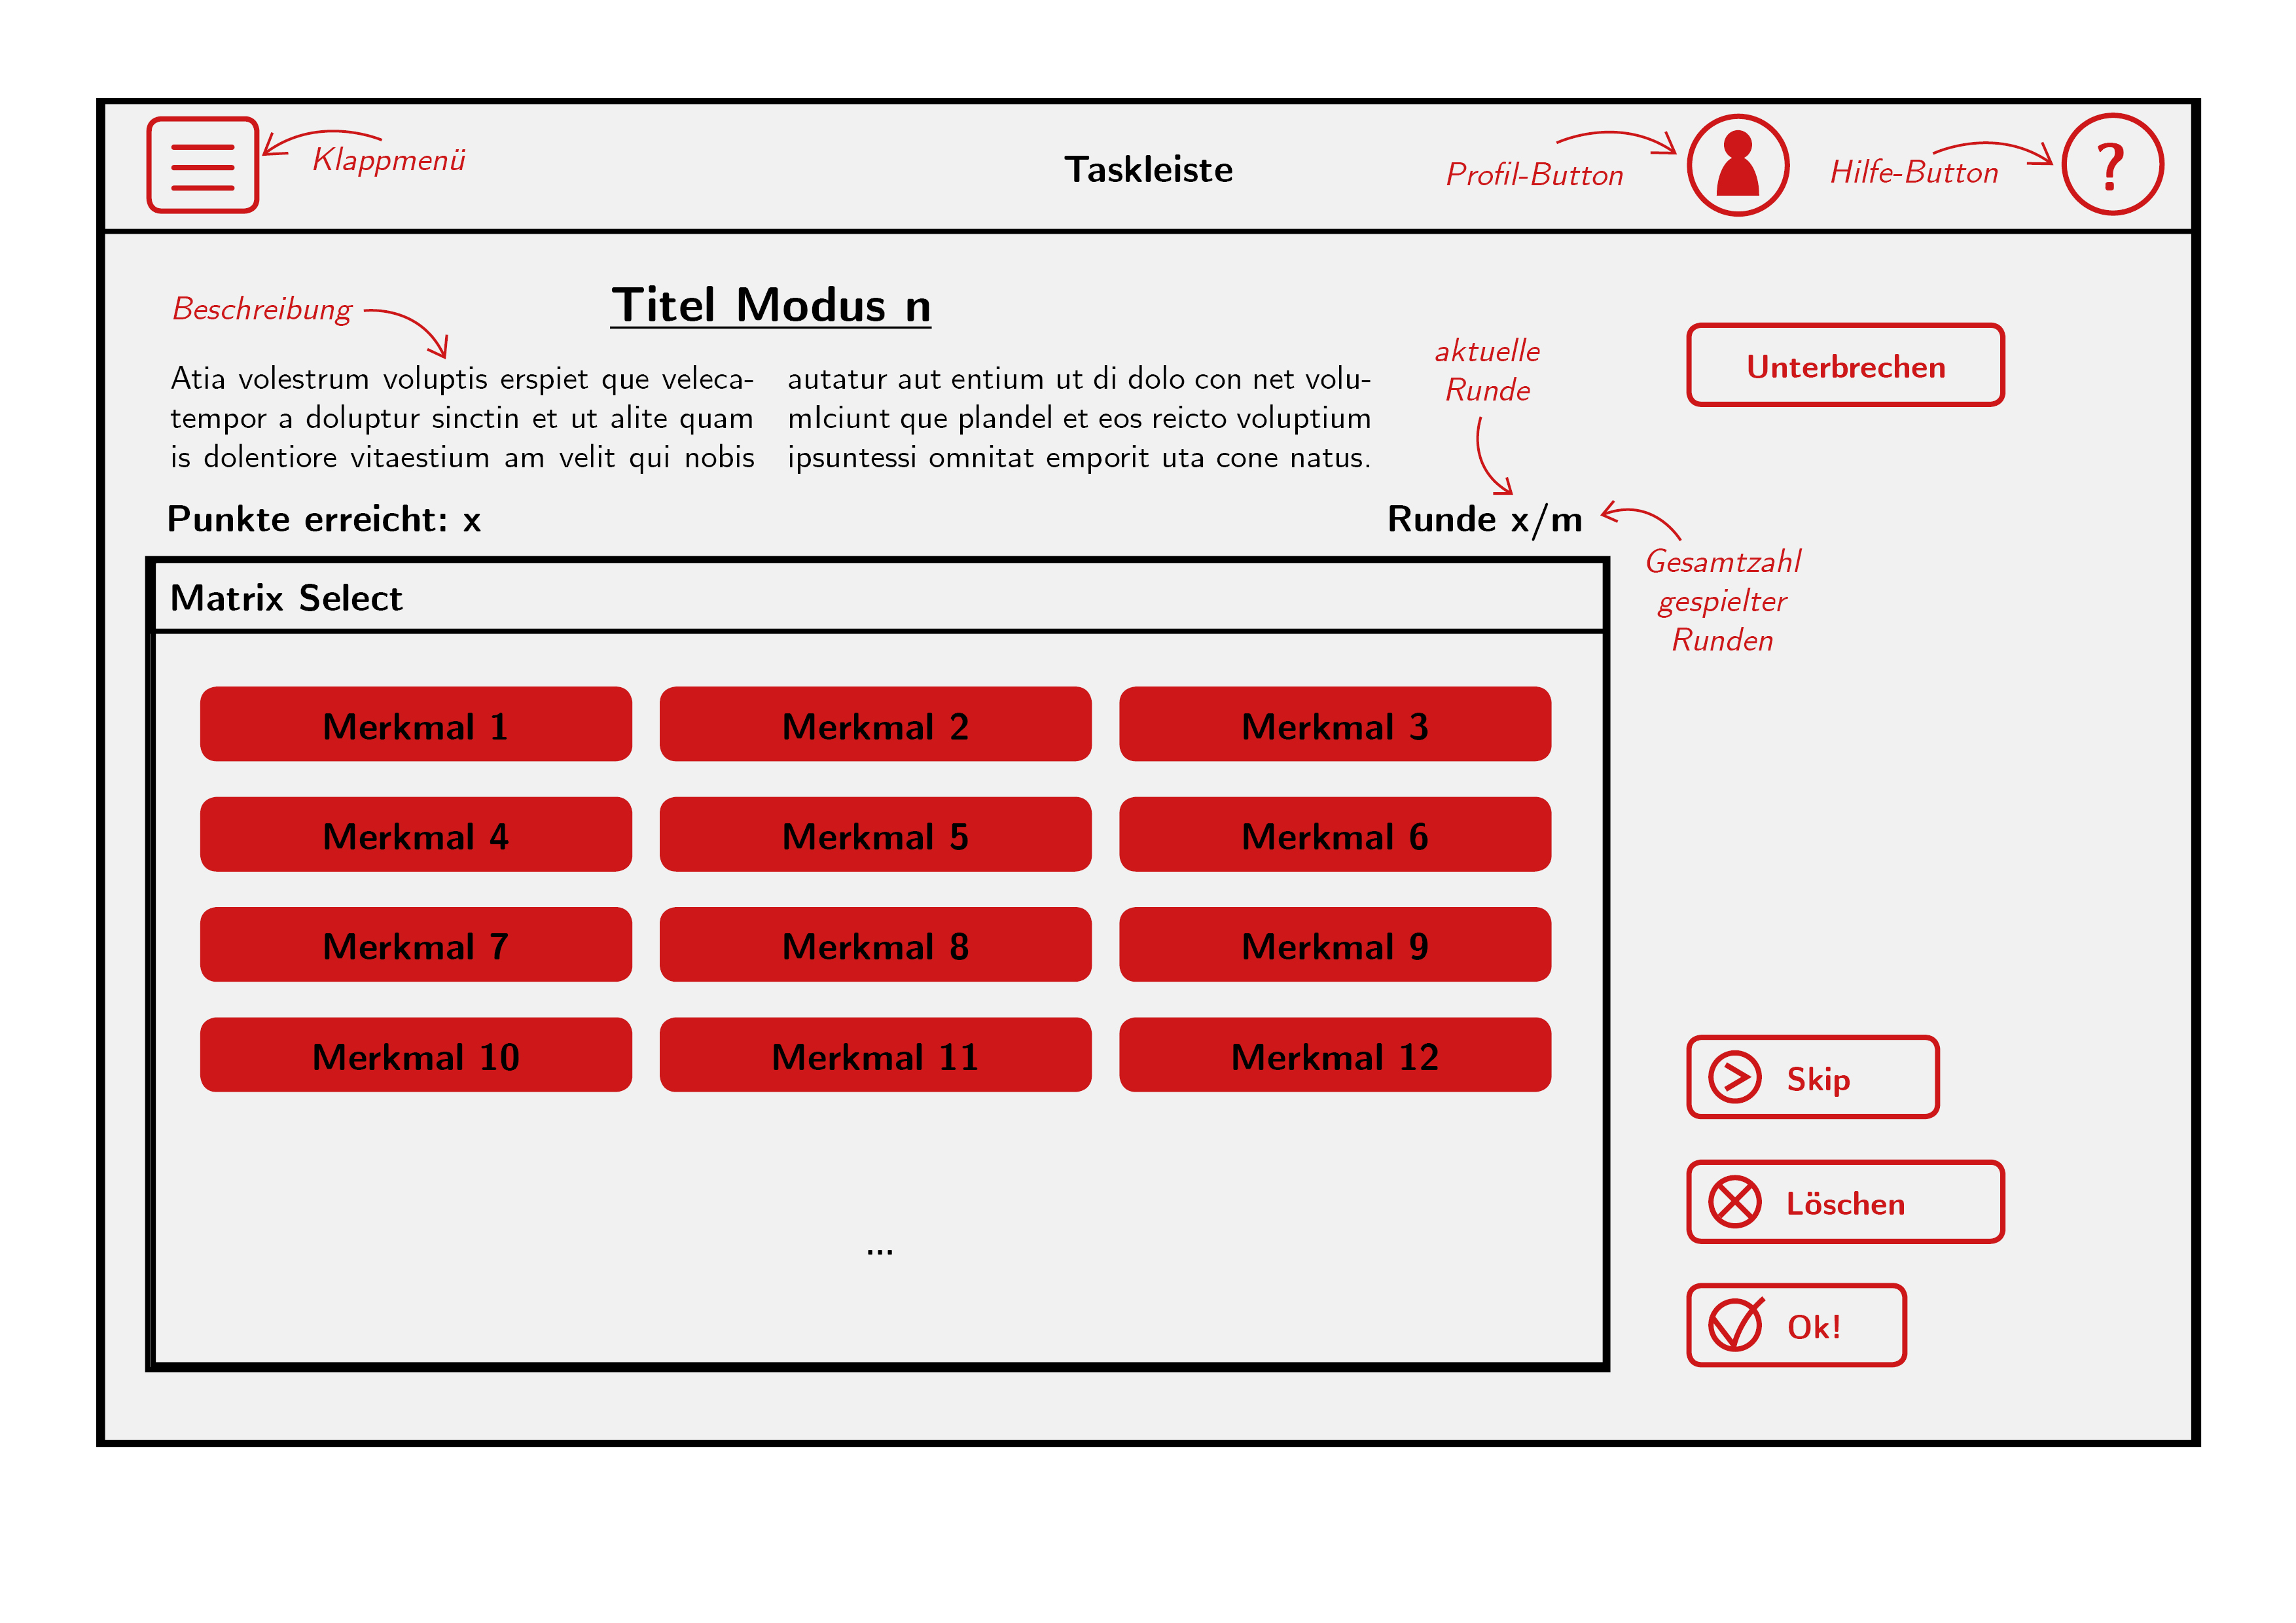
\includegraphics[width=\textwidth]{../../pictures/MatrixSelect.jpg}
	\end{frame}
	\begin{frame}
		\begin{block}{Binär Select spielen, Abmelden}
		Nun spielt der Spieler eine Runde des Spiels mit Spielmodus Binär Select und meldet sich anschließend ab.
		\end{block}
		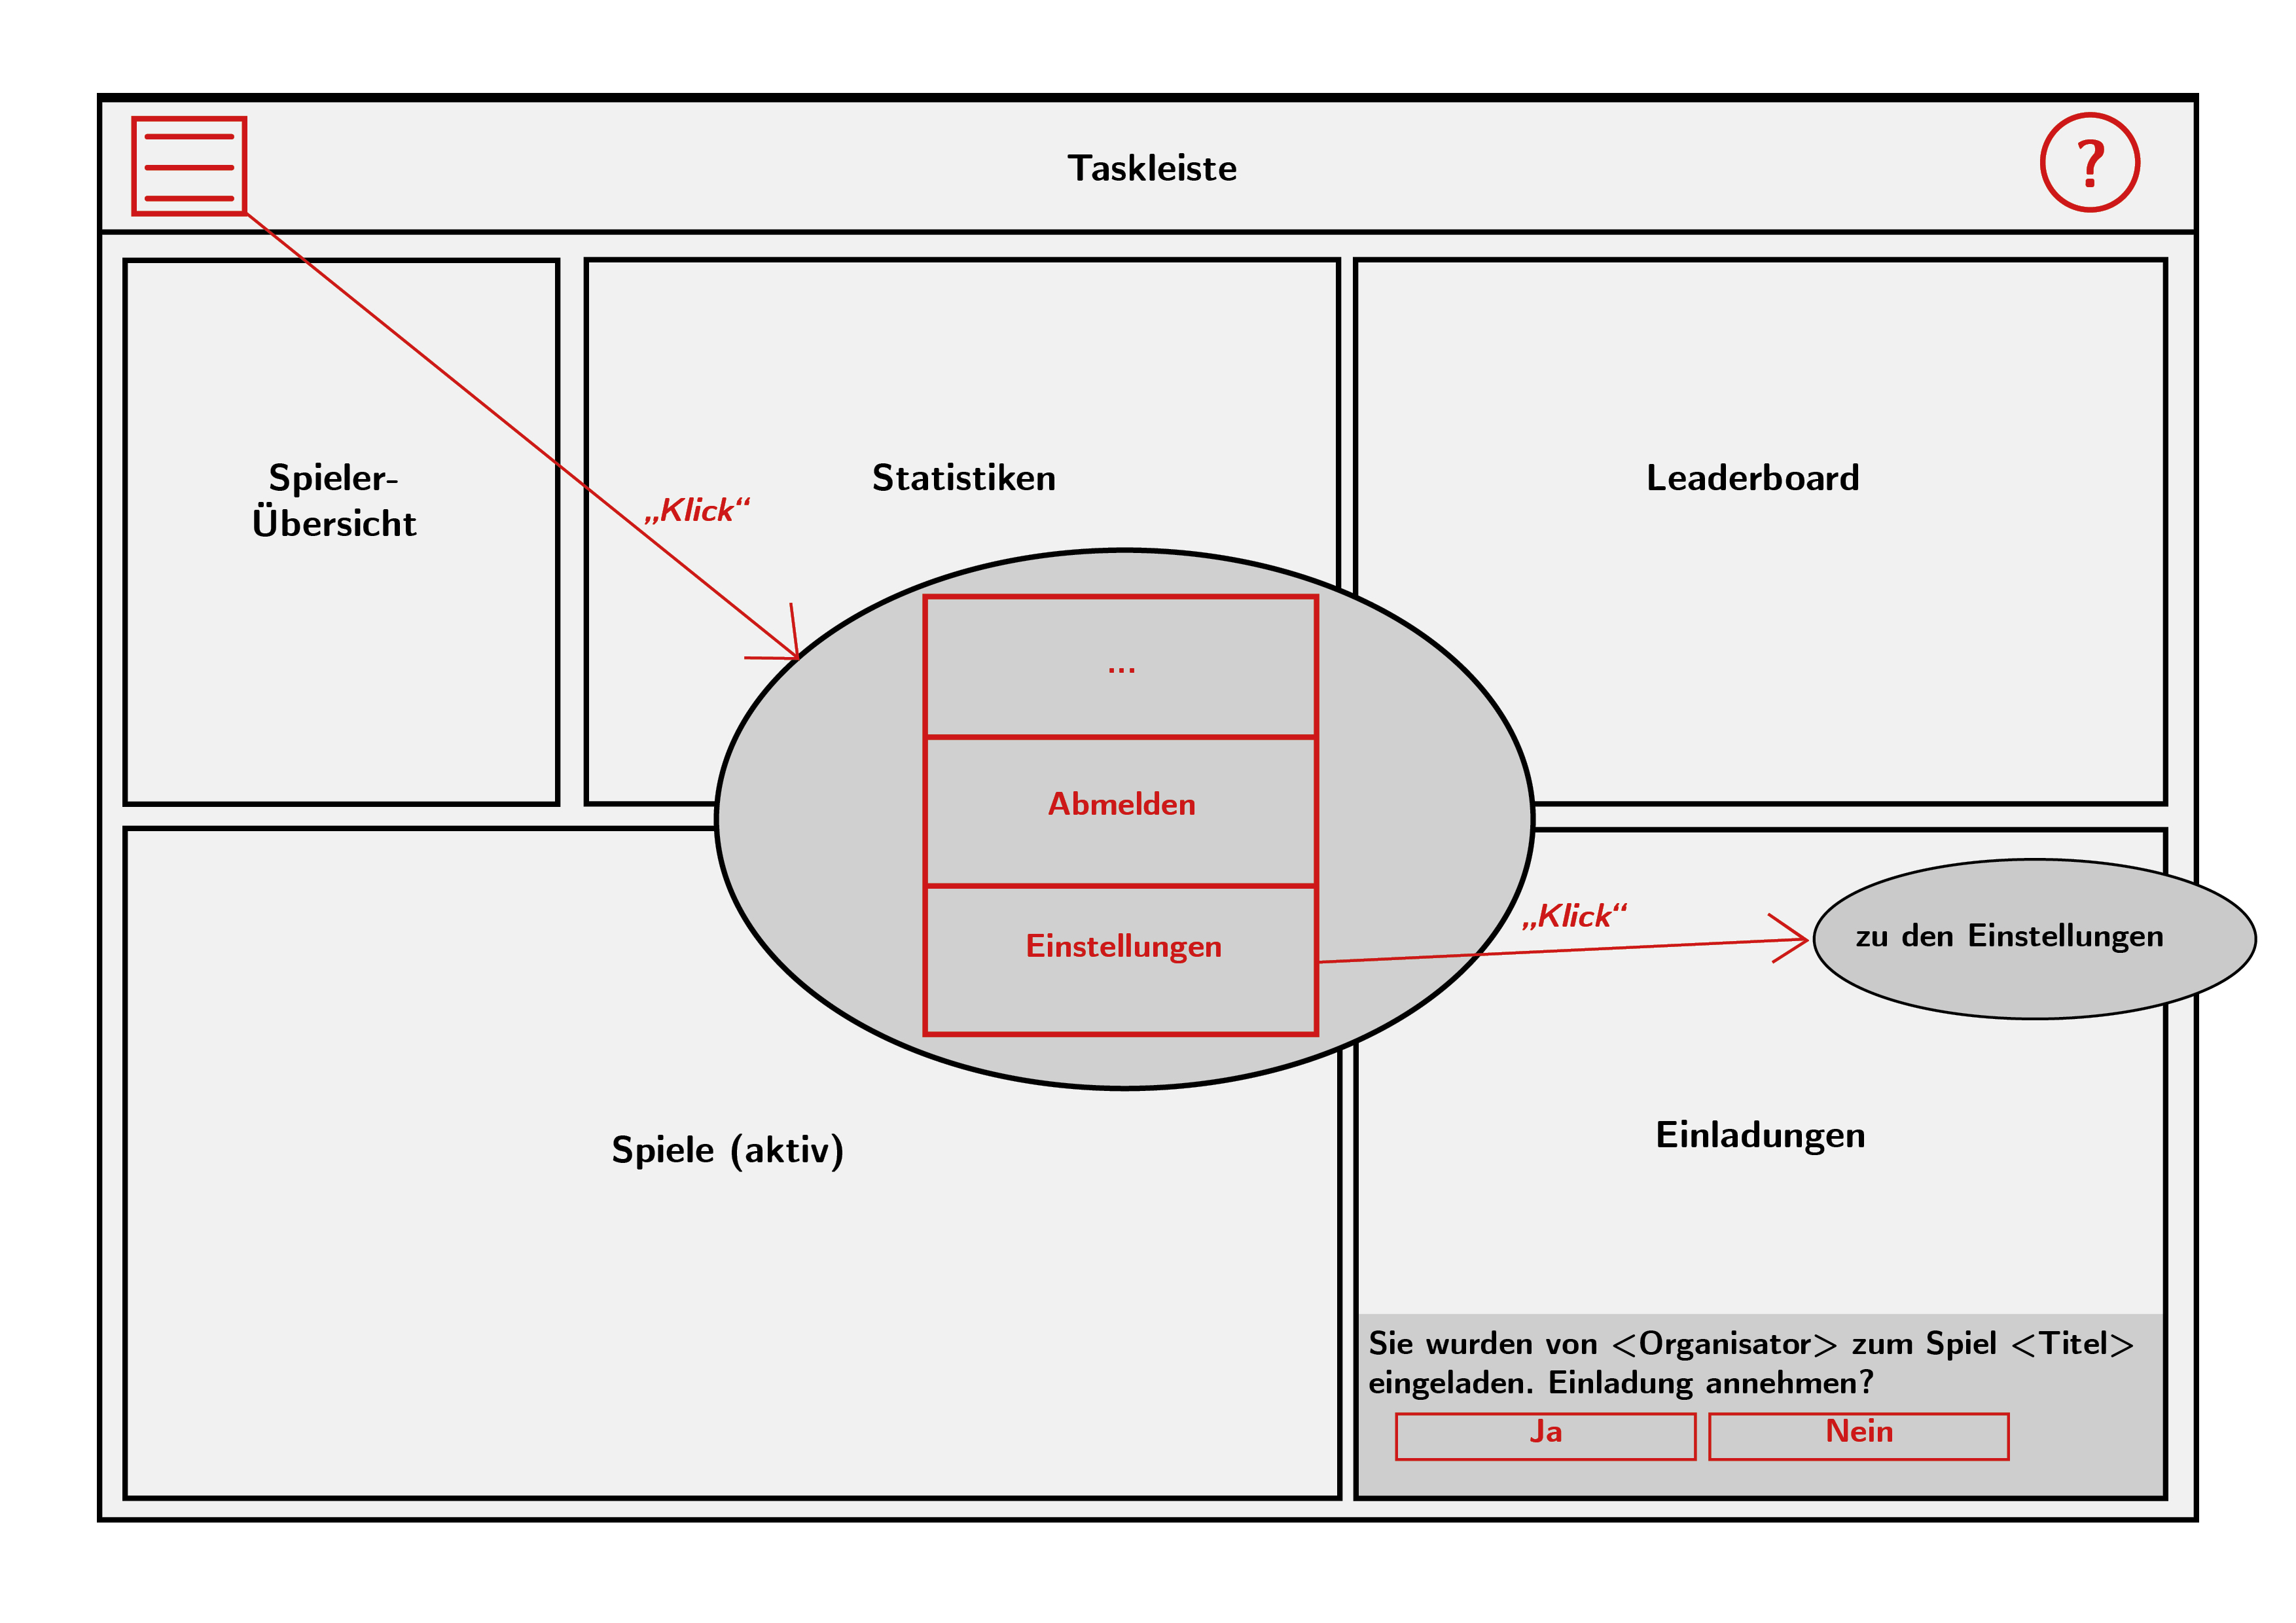
\includegraphics[width=8cm]{../../pictures/5_Spieler.jpg}
	\end{frame}
	\begin{frame}
	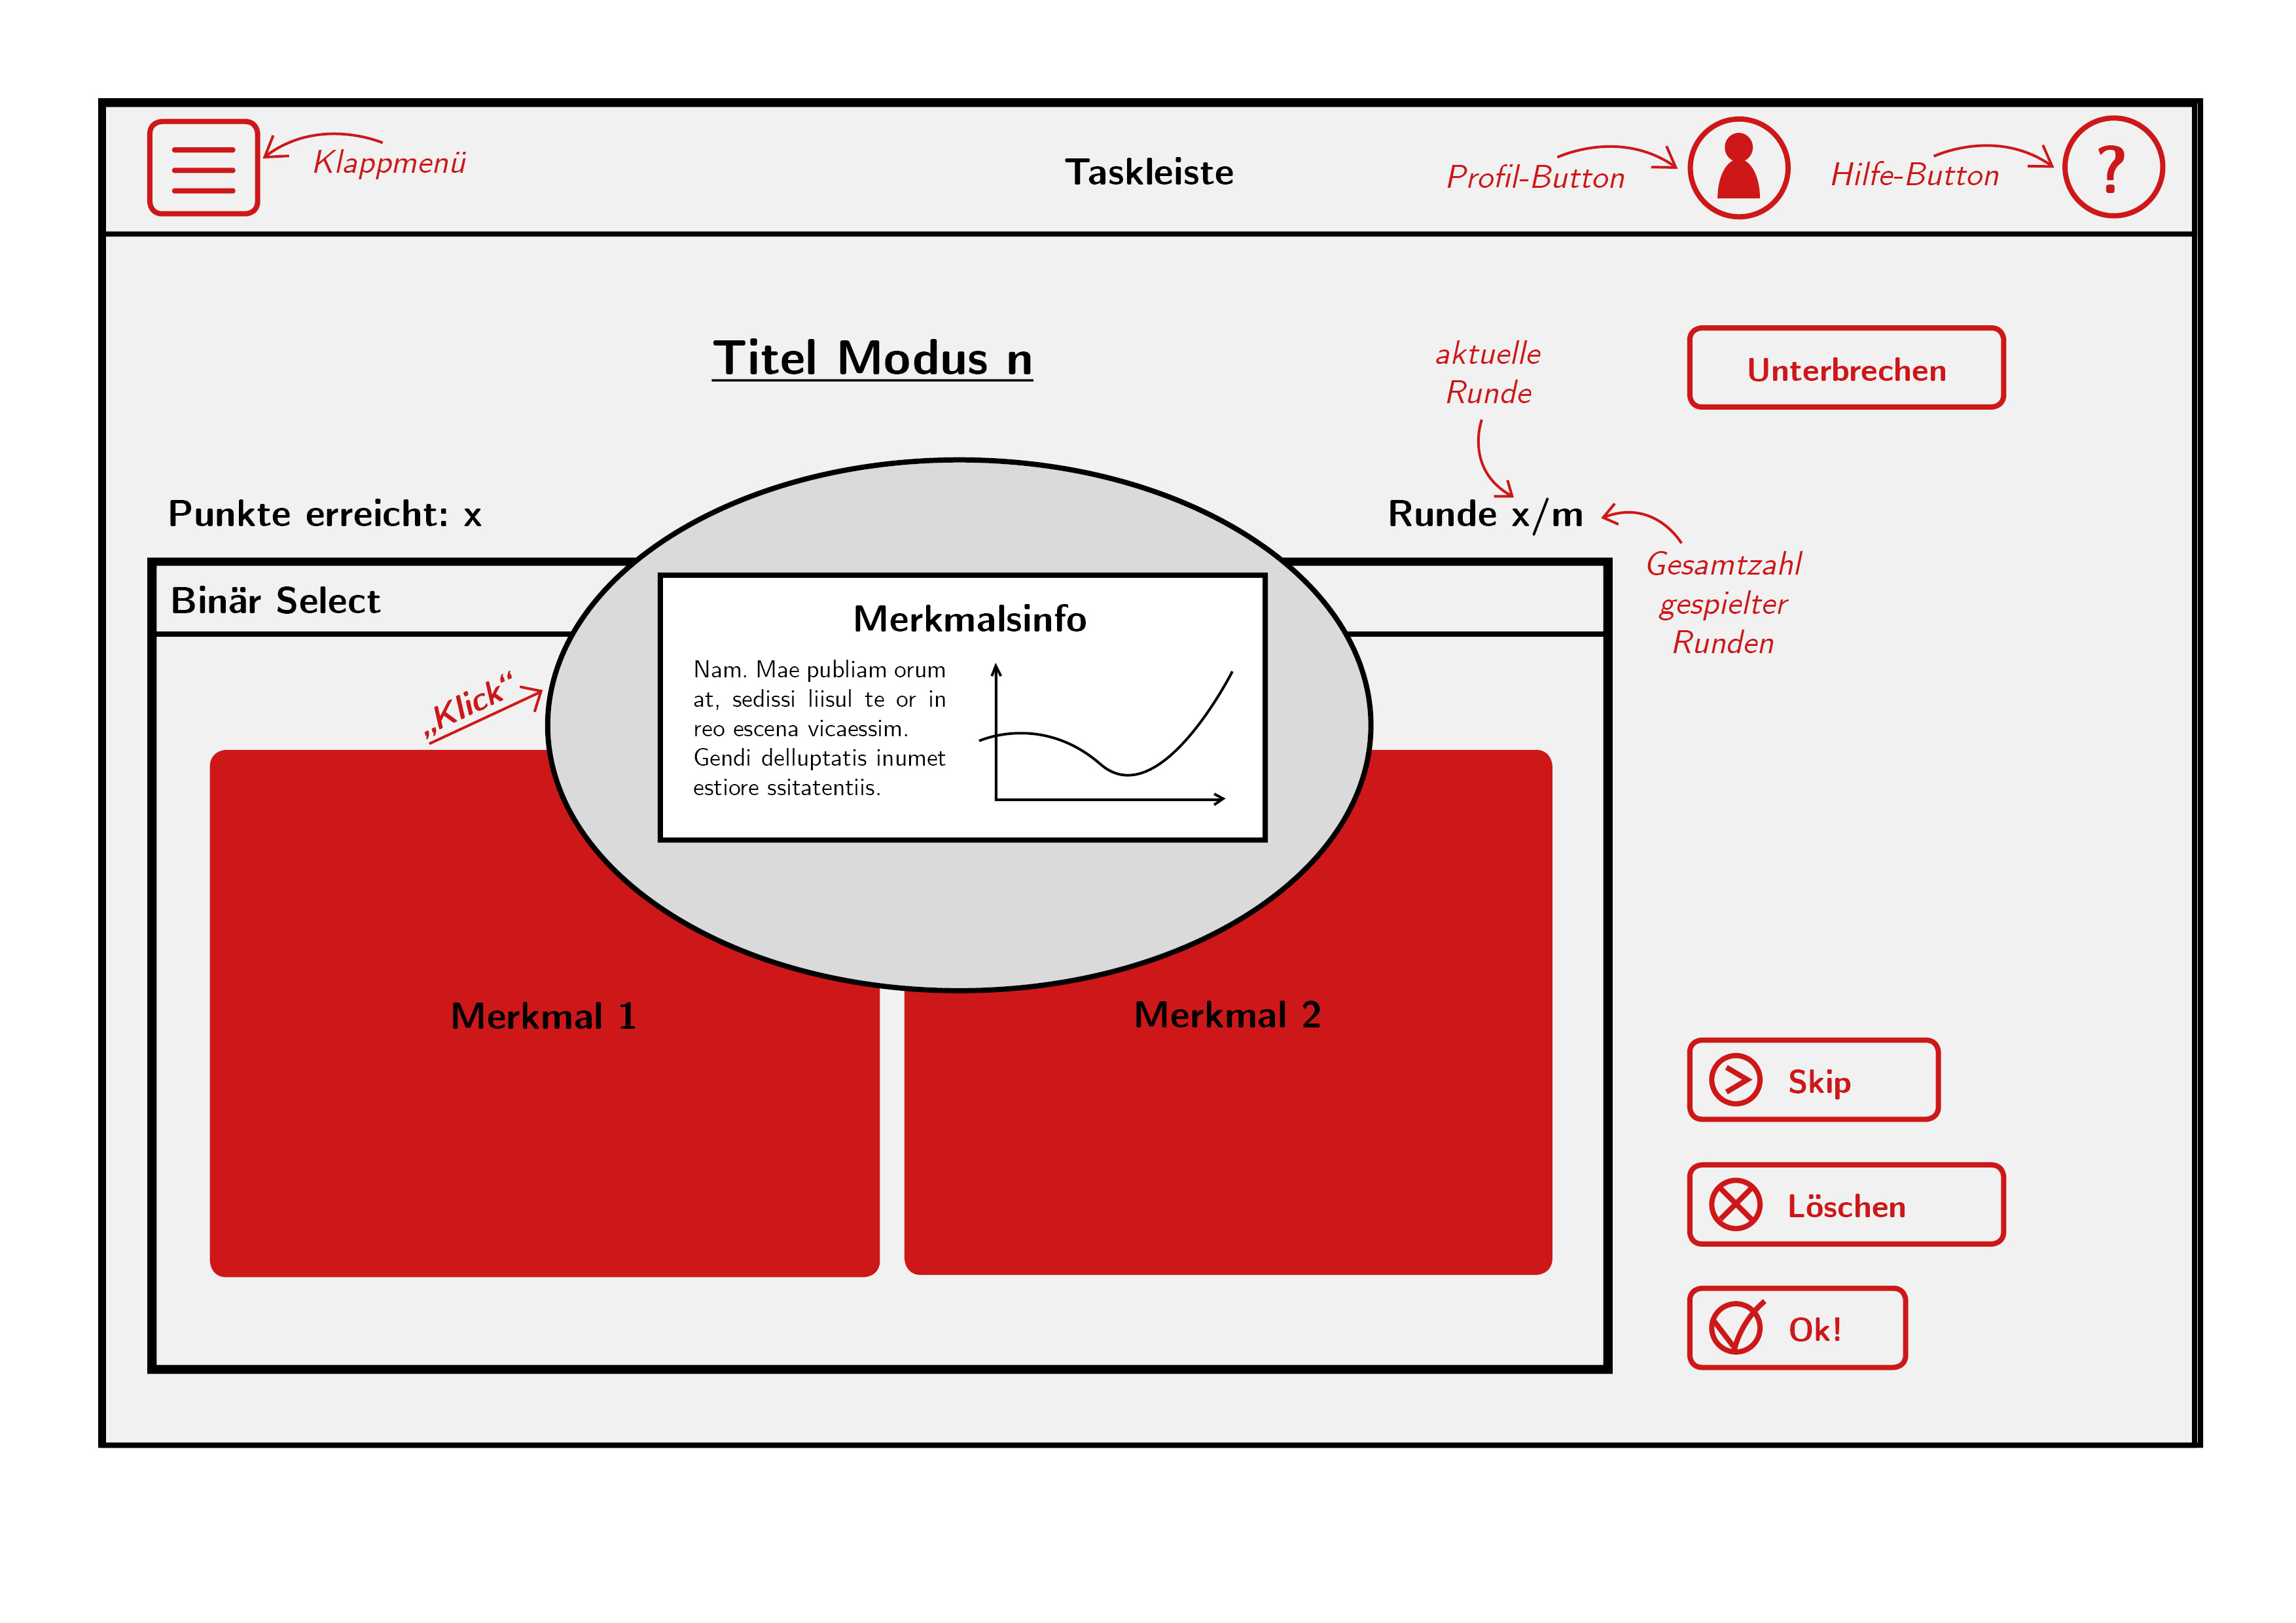
\includegraphics[width=\textwidth]{../../pictures/BinSelect.jpg}
	\end{frame}
	\begin{frame}
	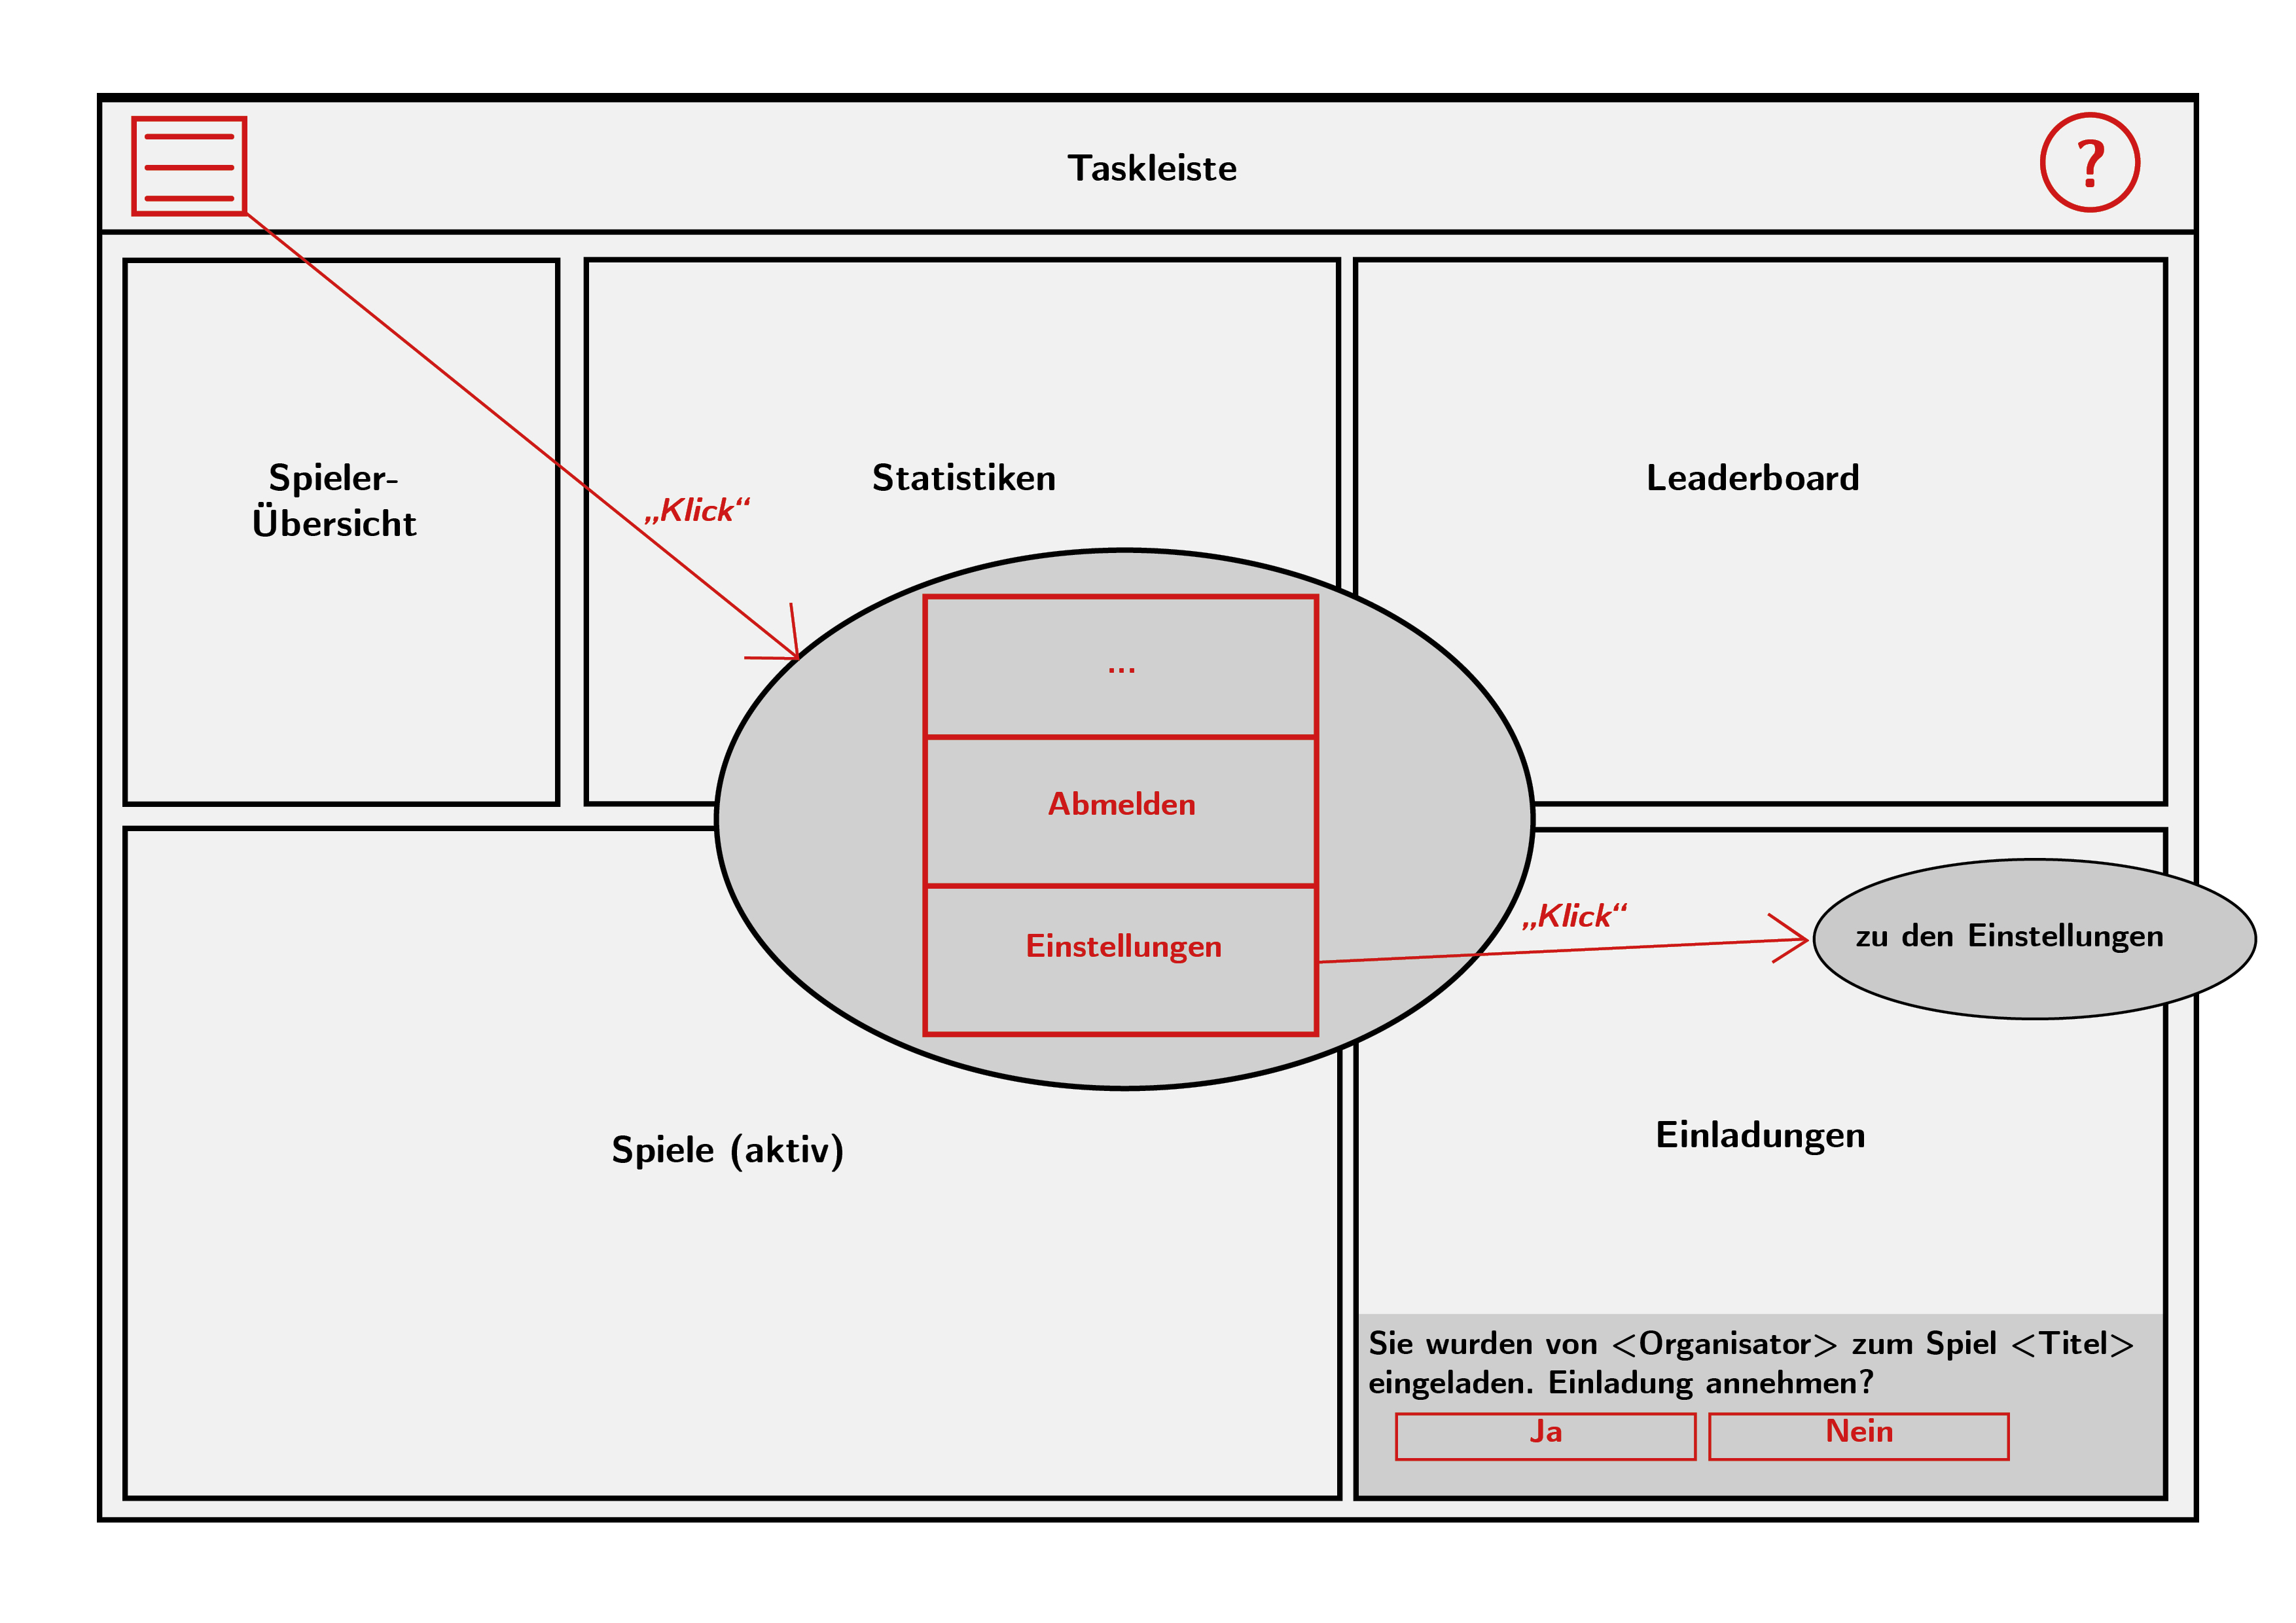
\includegraphics[width=\textwidth]{../../pictures/5_Spieler.jpg}
	\end{frame}
\end{document}
